\documentclass[12pt]{article}
\usepackage{graphicx, float}
\usepackage[utf8]{inputenc}
\usepackage[T2A]{fontenc}
\usepackage[serbianc]{babel}
\usepackage {amsmath, amssymb, amsthm}
\graphicspath{{figures/}}
\usepackage[shortlabels]{enumitem}
\usepackage{hyperref}
\hypersetup{colorlinks=true, linkcolor=black, urlcolor=blue, breaklinks=true}
\usepackage{xurl}
\usepackage{chngcntr}
\counterwithin{figure}{subsection}
\usepackage{caption}
\captionsetup{labelsep=space}
\usepackage{comment}
\usepackage{mathrsfs}
\newsavebox\foobox
\newlength{\foodim}
\newcommand{\slantbox}[2][0]{\mbox{%
        \sbox{\foobox}{#2}%
        \foodim=#1\wd\foobox
        \hskip \wd\foobox
        \hskip -0.5\foodim
        \pdfsave
        \pdfsetmatrix{1 0 #1 1}%
        \llap{\usebox{\foobox}}%
        \pdfrestore
        \hskip 0.5\foodim
}}
\def\Laplace{\slantbox[-.45]{$\mathscr{L}$}}

%   formatting
\usepackage[a4paper, top=1cm, bottom=2cm, left=2cm, right=1cm, heightrounded]{geometry}
\renewcommand{\baselinestretch}{1.15}
\usepackage{indentfirst}
\setlength{\parindent}{0cm}
\setlength{\parskip}{0.8em}

\title{Дипломски Рад}
\author{Лазар Попадић}
\date{Август 2024}
%\maketitle

\begin{document}
\tableofcontents
\newpage

\section{Увод}
У индустрији вођеној ефикасношћу и прецизношћу, све већа пажња се посвећује употреби паралелних манипулатора. У поређењу са серијским, паралелни манипулатори нуде значајне предности у погледу крутости, брзине, поновљивости као и ефикаснијег искоришћења енергије. Док серијски манипулатори пружају већу покретљивост, паралелни се истичу у задацима који захтевају велику носивост и прецизност, уз мање грешака услед деформација под оптерећењем. Ове карактеристике их чине посебно корисним у производним процесима, као што су \textit{pick-and-place} задаци, монтажа, прецизно позиционирање и оријентисање.
 Употреба глобалних оптимизационих алгоритама нам омогућава да пронађемо вредности управљачких параметара за које функција циља има оптималну вредност. Тек са таквим параметрима систем може да задовољи захтеване перформансе.

У овом раду се примењује \textit{Particle swarm optimization} алгоритам за пројектовање оптималног управљања петочланог паралелног манипулатора са 2 степена слободе. Показаћемо како минимизацијом функције циља, која зависи од грешке позиционирања улазних чланова и трзаја излазног члана, можемо добити параметре PID регулатора за које је кретање оптимално.
Овај рад је подељен на три дела.

Први део представља теоријску основу рада. Истакнута је анализа кретања паралелних манипулатора, модел машине једносмерне струје, основе PID регулације и принцип рада PSO алгоритма. 

У другом делу је детаљно приказана имплементација система, која подразумева динамички модел петочланог паралелног манипулатора укључујући и модел МЈС, имплементација регулационе петље и критеријум оптималности који се користи за оптимизацију. 

У трећем делу су приказани резултати оптимизације који су добијени симулацијом у \textit{MATLAB Simulink}-у. Приказан је и утицај параметара оптимизације, као и провера добијених параметара.

\newpage
\section{Материјали и Методе}

\subsection{Паралелни манипулатори}
Роботски манипулатори су уређаји који врше манипулацију објектима у простору. Главна функција манипулатора подразумева задатке који захтевају брзо и прецизно позиционирање предмета рада. Манипулатори су мехатроничарски уређаји који се састоје из механичког подсистема, управљачке и енергетске електронике. Према типу механичког подсистема, манипулатори се деле на: серијске, паралелне и мобилне.

Кинематски ланац представља низ крутих сегмената који су повезани преко зглобова. Прости кинематски ланци су они код којих ниједан сегмент није повезан са више од 2 сегмента. Механички подсистем серијских манипулатора представља прости кинематски ланац код којих су сегменти базе и крајњег ефектора повезани са 1, а сви остали са 2 сегмента [1]. Пример серијског манипулатора је приказан на слици 2.1.1.

\begin{figure}[H]
    \centering
    \includegraphics[width=12cm]{figures/abb_irb_140.jpg}
    \caption{Серијски манипулатор антропоморфне конфигурације \textit{ABB IRB} 140 [2]}
    \label{fig:серијски_манипулатор}
\end{figure}

Затворени кинематски ланац се добија када је један од сегмената, али не и база, повезан са 3 или више сегмента [1]. Механички подсистем паралелних манипулатора представља затворени кинематски ланац, код којег је крајњи ефектор повезан са базом преко више од једног кинематског ланца. Свака веза базе и крајњег ефектора садржи барем један актуатор. На слици 2.1.2 је приказан пример паралелног манипулатора.

\begin{figure}[H]
    \centering
    \includegraphics[width=12cm]{figures/abb_irb_360.jpg}
    \caption{Паралелни манипулатор делта конфигурације \textit{ABB IRB} 360 [2]}
    \label{fig:паралелни_манипулатор}
\end{figure}

За разлику од серијских, сви актуатори паралелних манипулатора могу бити на непокретном сегменту, односно бази. То омогућава да, без негативних последица на крутост ланца, сегменти буду лакши него код серијских манипулатора. Додатна предност је то што се оптерећење које делује на крајњи ефектор разлаже на сваки ланац којим је повезан са базом. Из тога закључујемо да су главне предности паралелних манипулатора у односу на серијске:
\begin{itemize}
    \item већа крутост кинематског ланца
    \item мања маса манипулатора
    \item већа носивост
    \item боља прецизност, као последица мањих деформација
\end{itemize}
С обзиром на то да је код паралелних манипулатора крајњи ефектор повезан са базом преко више од 1 кинематског ланца, кинематска анализа је знатно сложенија. Такође, сваки кинематски ланац уноси и одређена кинематска ограничења, због којих је радни простор мањи него код серијских манипулатора. 
Главне мане паралелних манипулатора су:
\begin{itemize}
    \item мањи радни простор
    \item сложенија кинематска и динамичка анализа
\end{itemize}

\subsubsection{Сингуларне конфигурације}
Сингуларне конфигурације су одређени положаји крајњег ефектора, за које паралелни роботи губе своју инхерентну бесконачну крутост, и у којима крајњи ефектор има неконтролисане степене слободе.[1] Типови кинематских сингуларитета су:
\begin{itemize}
    \item Тип 1. За ненулти вектор улазних брзина, крајњи ефектор се не креће.
    \item Тип 2. Крајњи ефектор се креће при нултом вектору улазних брзина.
    \item Тип 3. Комбинација сингуларитета типа 1 и 2. Могуће је кретање крајњег ефектора без кретања улазних сегмената, и обрнуто, могуће је кретање улазних сегмената без кретања крајњег ефектора.
\end{itemize}

\subsubsection{Кинематска анализа}
Кинематска анализа манипулатора обухвата проучавање кретања свих сегмената. Од кључног значаја су односи између координата, брзина и убрзања улазних чланова и крајњег ефектора. Кинематски проблем се дели на директни и индиректни.

Директни кинематски проблем обухвата проналажење кинематских параметара крајњег ефектора за задате улазне параметре кретања. Решење за паралелне манипулаторе зависи од конфигурације, односно, не мора бити јединствено. Аналитичка метода за решавање проблема директне кинематике представља решавање система векторских једначина. Почевши од система за положај, формулишу се векторске једначине које изражавају вектор положаја врха крајњег ефектора преко карактеристичних вектора. Карактеристични вектори описују положај једног сегмента кинематског ланца. Карактеристични вектор је постављен у правцу сегмента, а његов интензитет представља дужину тог сегмента.

Након решавања система за положај, векторске једначине се диференцирају по времену како би се добио систем за брзину. Након тога се опет диференцирају како би се добио систем за убрзање. Слика 2.1.3 приказује директан кинематски проблем за зглобни четвороугао.

\begin{figure}[H]
    \centering
    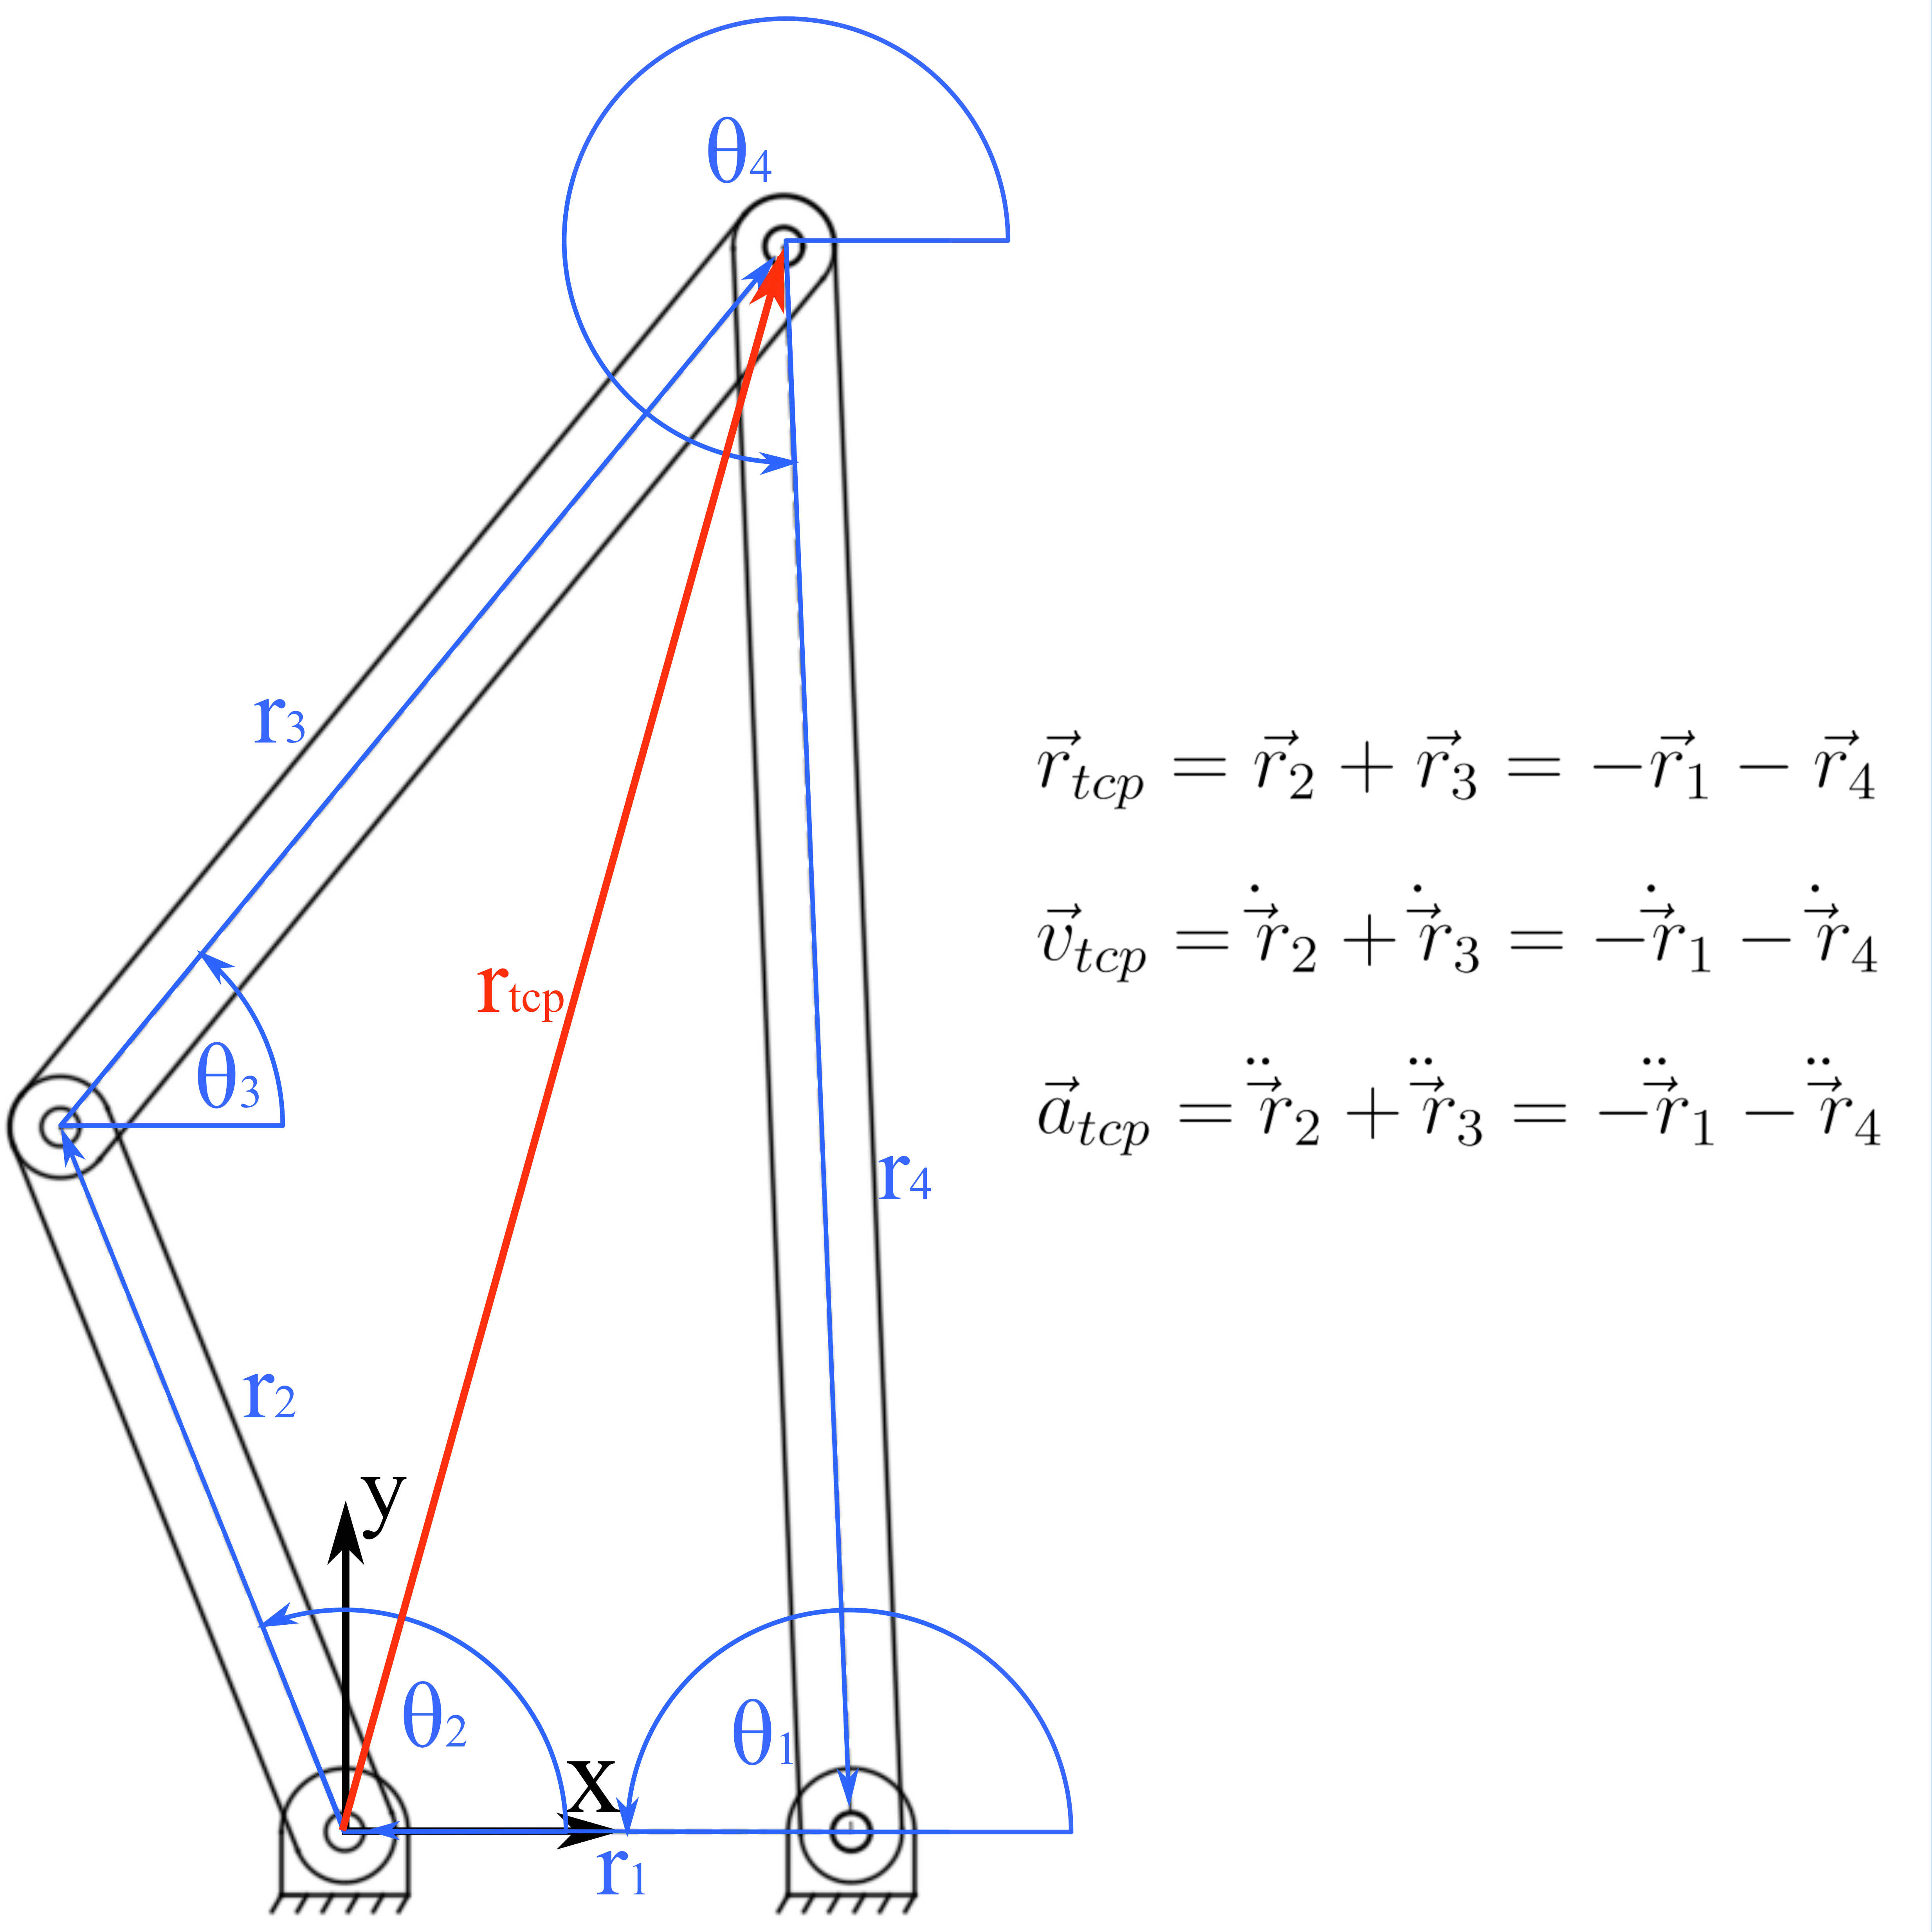
\includegraphics[width=7cm]{figures/4bar.jpg}
    \caption{Пример директног кинематског проблема}
    \label{fig:дир_кин_пример}
\end{figure}

Инверзни кинематски проблем обухвата проналажење параметара улазних сегмената за жељени положај крајњег ефектора. Као и код директног, решење не мора бити јединствено. Иста метода за решавање директне кинематике се може применити и за инверзну кинематику.

\subsubsection{Динамичка анализа}
Динамичка анализа представља одређивање односа између кинематских параметара и оптерећења која делују на манипулатор. Динамика обухвата постављање једначина кретања, које описују како се манипулатор креће под утицајем оптерећења. Оптерећења могу бити спољашња и унутрашња. Спољашња настају услед утицаја спољашњих сила и момената, на пример гравитациона сила предмета рада и силе улазних актуатора. Унутрашња оптерећења обухватају реакције веза у зглобовима кинематског ланца.

Једначине кретања могу бити исписане помоћу Њутн-Ојлерових једначина кретања. Оне су допуњене Даламберовим принципом који уводи инерцијалну силу: $\vec{F}_{in} - m\vec{a} = 0,$ и инерцијални момент силе: $\vec{M}_{in} - I\vec{\alpha} = 0$. Даламберов принцип нам омогућава да динамичке проблеме посматрамо као статичке [3].

Динамичка анализа обухвата директан и инверзни динамички проблем. Директан проблем обухвата израчунавање трајекторије, брзине и убрзања крајњег ефектора на основу задатих улазних оптерећења. Инверзан проблем обухвата израчунавање потребних улазних оптерећења на основу задате трајекторије, брзине и убрзања крајњег ефектора.

Решавање проблема динамике обухвата вршење декомпозиције кинематског ланца, односно формирање \textit{Free-Body Diagram}-а. Затим се формирају једначине кретања за ротационо и транслаторно кретање сваког сегмента. Притом сила реакције везе којом један сегмент делује на други је истог интензитета и правца, а супротног смера у односу на силу којом тај други сегмент делује на први, на пример: $\vec{F_{12}} = -\vec{F_{21}}$. Формирањем тих једначина добија се систем, чије решење представља решење динамичког проблема[4]. Пример \textit{Free-Body Diagram}-а за зглобни четвороугао је приказан на слици 2.1.4.

\begin{figure}[H]
    \centering
    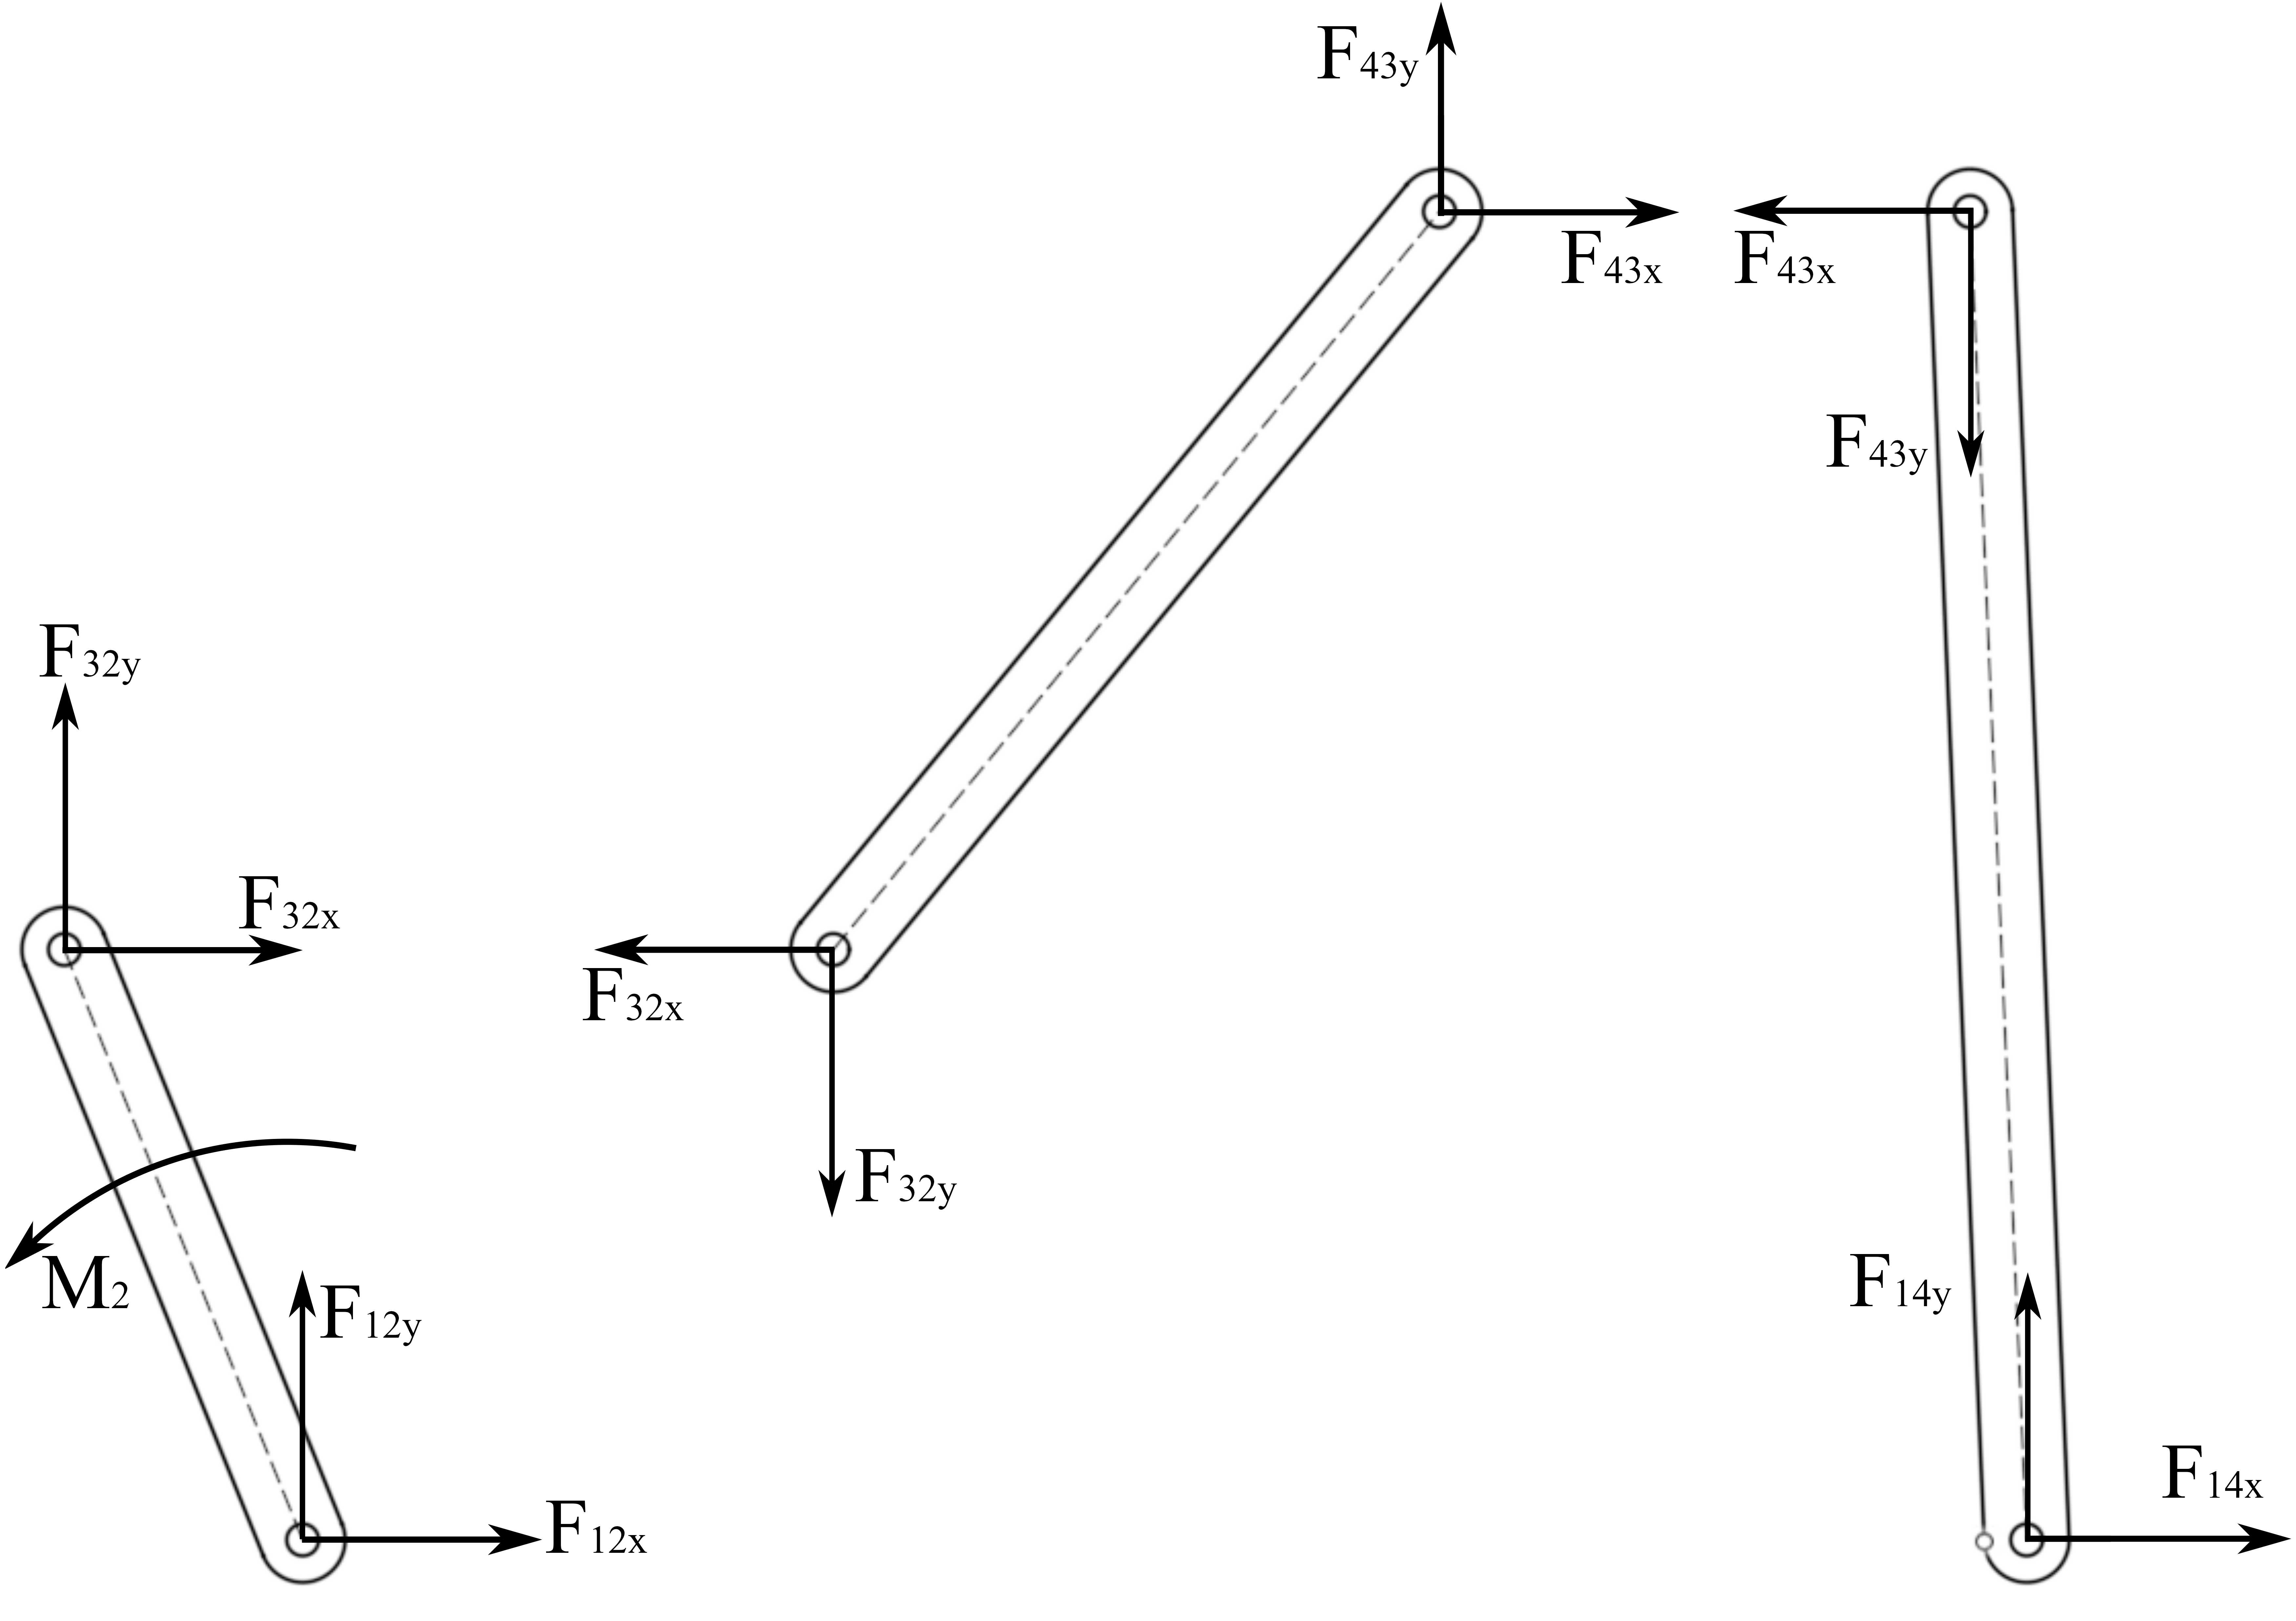
\includegraphics[width=12cm]{figures/4bar_fbd.jpg}
    \caption{Пример \textit{Free-Body Diagram}-а}
    \label{fig:фбд_пример}
\end{figure}

\subsection{Машине једносмерне струје}
Машине једносмерне струје, у наставку МЈС, су електромеханички претварачи, који улазну електричну енергију претварају у механички рад. Састоје се из статора и ротора(арматуре). Статор успоставља побудно магнетно поље, због чега се назива и побуда. Кроз ротор се, преко четкица и комутатора, пропушта улазна арматурна струја. По принципу Лоренцовог закона $\vec F=Q(\vec v \times \vec B)$, индукује се сила која делује на ротор. Комутатор врши промену смера арматурне струје у зависности од положаја ротора, и тиме омогућава да Лоренцова сила увек делује у истом смеру, односно обезбеђује константан обртни момент мотора. Због Фарадејевог закона и Ленцовог правила $e_a=-N\dfrac{\partial\phi }{\partial t}$, обртање ротора индукује електромоторну силу супротног смера. Слика 2.2.1 приказује еквивалентно коло арматурног намотаја.

\begin{figure}[H]
    \centering
    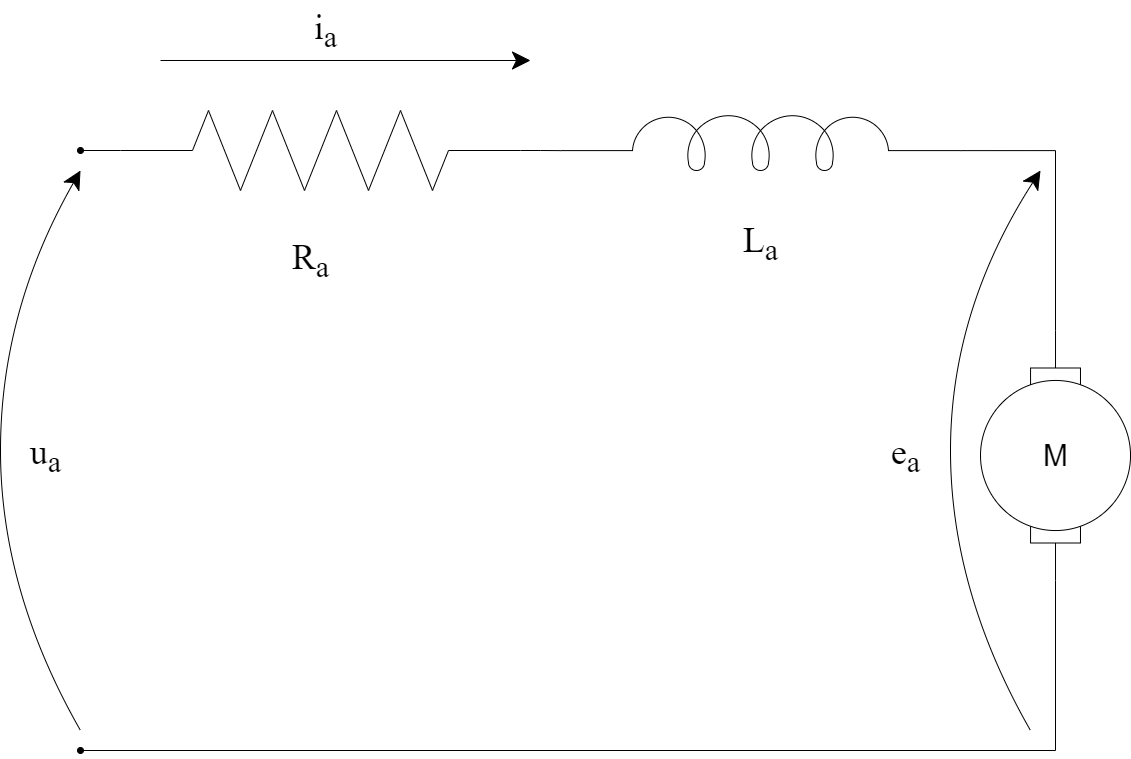
\includegraphics[width=12cm]{figures/ekv_kolo_armatura.png}
    \caption{Еквивалентно коло арматуре МЈС}
    \label{fig:коло_арматуре}
\end{figure}


\subsubsection{Динамички модел МЈС}
Модел МЈС се састоји из 2 подсистема: механичког и електричног, који међусобно интерагују. Посматраћемо МЈС која има сталну побуду јачинe магнетног флукса $\psi _f$. Модел се састоји из 3 диференцијалне једначине: напонске равнотеже арматурног намотаја, механичке равнотеже и релације механичке брзине обртања и угла ротора, као и из 2 алгебарске једначине: дефиниције електромагнетног момента и дефиниције индуковане електромоторне силе [5].
\begin{equation}
    u_a-e_a=R_ai_a+L_a\dfrac{di_a}{dt}
\end{equation}
\begin{equation}
    m_e-m_m=J_m \dot\omega+B_m\omega
\end{equation}
\begin{equation}
    \dfrac{d\theta}{dt}=\omega
\end{equation}
\begin{equation}
    m_e=\psi _fi_a
\end{equation}
\begin{equation}
    e_a=\psi _f\omega
\end{equation}
%\newpage
Значења величина математичког модела МЈС су:
\begin{itemize}
    \item $u_a\;$ - улазни арматурни напон
    \item $e_a\;$ - индукована електромоторна сила
    \item $R_a\;$ - електрична отпорност арматурног намотаја
    \item $i_a\;$ - арматурна струја
    \item $L_a\;$ - индуктивност арматурног намотаја
    \item $m_e\;$ - електромагнетни момент
    \item $m_m\;$ - момент оптерећења
    \item $J_m\;$ - момент инерције обртних маса
    \item $\omega\;$ - угаона брзина арматуре
    \item $B_m\;$ - коефицијент пригушења брзине услед трења
    \item $\theta\;$ - угао ротора
    \item $\psi _f\;$ - јачина магнетног флукса побуде
\end{itemize}

\subsubsection{МЈС у стационарном стању}
Стационарно стање МЈС подразумева режим рада у којем су изводи променљивих стања по времену једнаки нули, односно, арматурни напон и струја, момент оптерећења и угаона брзина су константни. Овакво стање система је равнотежно и омогућава нам да лакше увидимо законитости утицаја улазних величина на излазне. Из једначина (2) и (4) следи:
\begin{equation}
    i_a=\dfrac{B_m\omega+m_m}{\psi _f}
\end{equation}
Уврштавањем (5) и (6) у (1) добијамо:
\begin{equation}
    \omega(1+\dfrac{R_aB_m}{\psi _f^2})=\dfrac{u_a}{\psi _f}-\dfrac{R_am_m}{\psi _f^2}
\end{equation}
Коефицијент пригушења брзине $B_m$ је типично занемарљив [6], због чега уводимо апроксимацију $B_m=0$. Тиме (6) и (7) постају:
\begin{equation}
    i_a=\dfrac{m_m}{\psi _f}
\end{equation}
\begin{equation}
    \omega=\dfrac{u_a}{\psi _f}-\dfrac{R_am_m}{\psi _f^2}
\end{equation}
Из (9) се може закључити да повећањем арматурног напона, угаона брзина линеарно расте, а повећањем момента оптерећења угаона брзина линеарно опада. Из тог закључка следи и идеја о регулацији брзине МЈС променом улазног арматурног напона [7]. Механичка карактеристика за номиналне вредности арматурног напона се назива природна карактеристика, и приказана је на слици 2.2.2. На истој слици је приказана карактеристика при нижем напону.

\begin{figure}[H]
    \centering
    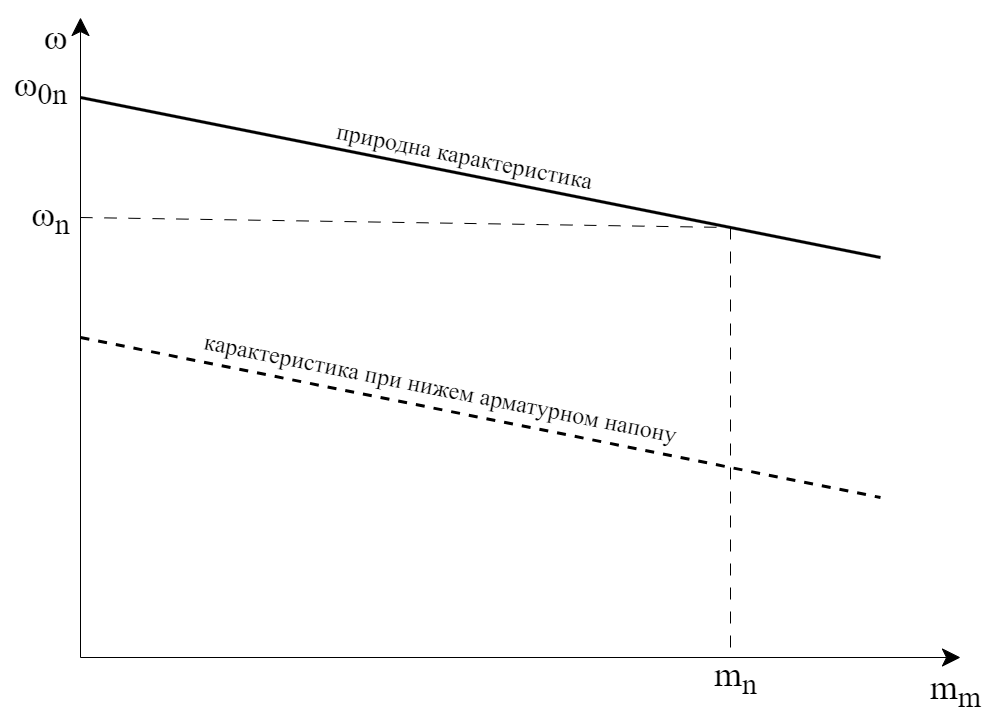
\includegraphics[width=15cm]{figures/k-ka_bdc.drawio.png}
    \caption{Механичка карактеристика МЈС}
    \label{fig:карактеристика_мјс}
\end{figure}

\subsection{PID регулација}
Регулација процеса представља управљање променљивима од значаја на основу управљачког алгоритма. Управљачки алгоритам представља функцију на основу које се генерише управљачки сигнал. Основни захтеви регулације су: стабилност, тачност и брзина одзива. Два основна типа регулације су у затвореној и отвореној петљи, односно, управљање са повратном спрегом и без повратне спреге. 

Регулација у отвореној петљи (open-loop control, non-feedback control loop) представља управљање у којем вредности излазних сигнала и сметњи немају утицај на управљачке сигнале. Овакви системи немају могућност отклањања грешака које су настале услед спољашњих поремећаја који делују на систем, или услед неидеалног познавања функционисања система. Системи који користе регулацију у отвореној петљи су спори системи који не захтевају велику прецизност и поновљивост. Слика 2.3.1 показује основну блок шему управљања у отвореној спрези.

\begin{figure}[H]
    \centering
    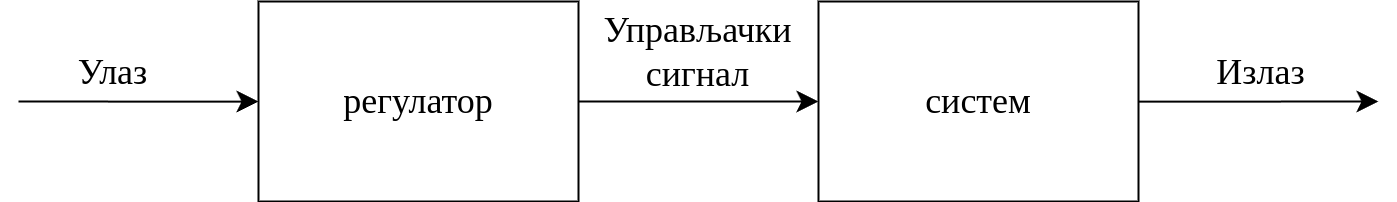
\includegraphics[width=14cm]{figures/open_loop.drawio.png}
    \caption{Блок шема управљања у отвореној спрези}
    \label{fig:отворена_спрега}
\end{figure}

Регулација у затвореној петљи (closed-loop control, feedback control loop) представља управљање у којем вредност управљачких сигнала зависи од разлике референтне(жељене) вредности и измерене вредности излазног сигнала. Овакви системи не захтевају идеално познавање управљаног система и имају могућност отклањања грешака услед спољашњих поремећаја. Слика 2.3.2 показује блок шему управљања у затвореној спрези.

\begin{figure}[H]
    \centering
    \includegraphics[width=15cm]{figures/closed_loop.jpg}
    \caption{Блок шема управљања у затвореној спрези}
    \label{fig:затворена_спрега}
\end{figure}

\subsubsection{Пропорцијално дејство}
Регулација на основу пропорцијалног дејства, односно P регулатори, представљају најједноставнији тип регулације са затвореном повратном спрегом. Управљачки сигнал је сигнал грешке помножен фактором појачања пропорцијалног дејства[8]:
\begin{equation}
    u_{(t)} = K_p e_{(t)},
\end{equation}
где $K_p$ представља фактор појачања пропорцијалног дејства, $u_{(t)}$ је управљачки сигнал, а $e_{(t)}$ је сигнал грешке. Сигнал грешке је једнак разлици референтне вредности и измерене вредности излаза, односно:
\begin{equation}
    e_{(t)}=y_{ref(t)} - y_{mer(t)}
\end{equation}
Функција преноса P регулатора у комплексном домену је:
\begin{equation}
    G_{p(s)} = \dfrac{U_{(s)}}{E_{(s)}} = K_p
\end{equation}
При одскочном сигналу грешке, одзив P регулатора изгледа као на слици 2.3.3.
\begin{figure}[H]
    \centering
    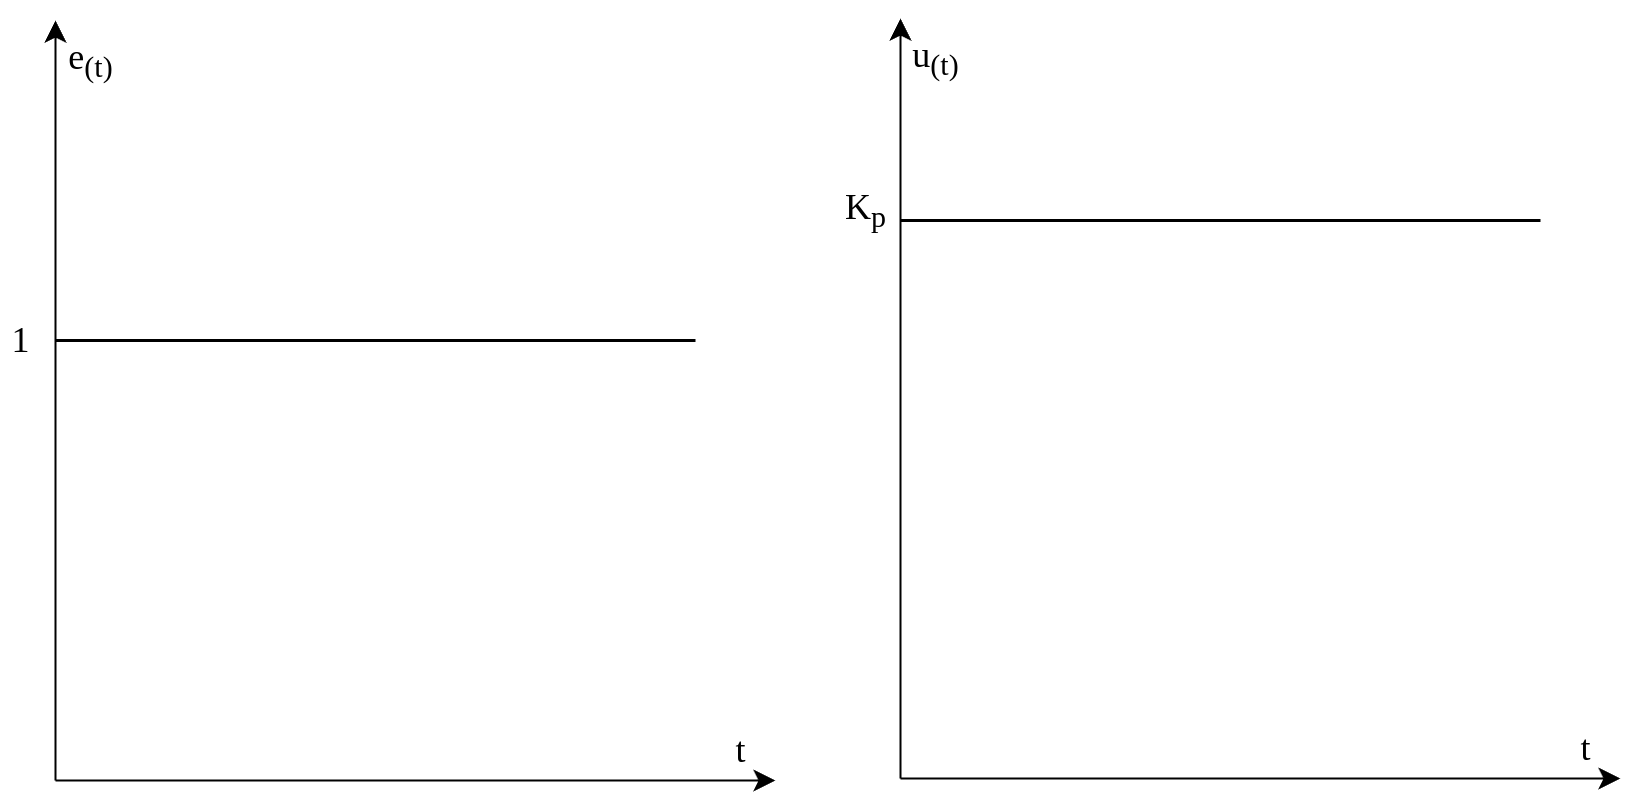
\includegraphics[width=13cm]{figures/p.drawio.png}
    \caption{Одзив P регулатора на одскочни сигнал грешке}
    \label{fig:P_одзив}
\end{figure}

\subsubsection{Интегрално дејство}
Регулација на основу интегралног дејства, односно I регулатори, су настали како би отклонили главну ману P регулатора. Та мана је немогућност потпуног отклањања грешке у стационарном стању. I дејство негативно утиче на брзину одзива и на стабилност система. Управљачки сигнал I регулатора представља одређен интеграл сигнала грешке по времену, помножен фактором појачања интегралног дејства $K_i$[8]:
\begin{equation}
    u_{(t)} = K_i\int_{0}^{t}e_{(t)}dt
\end{equation}
Функција преноса I регулатора у комплексном домену је:
\begin{equation}
    G_{i(s)} = \dfrac{U_{(s)}}{E_{(s)}} = \dfrac{K_i}{s}
\end{equation}
При одскочном сигналу грешке, одзив I регулатора изгледа као на слици 2.3.4.
\begin{figure}[H]
    \centering
    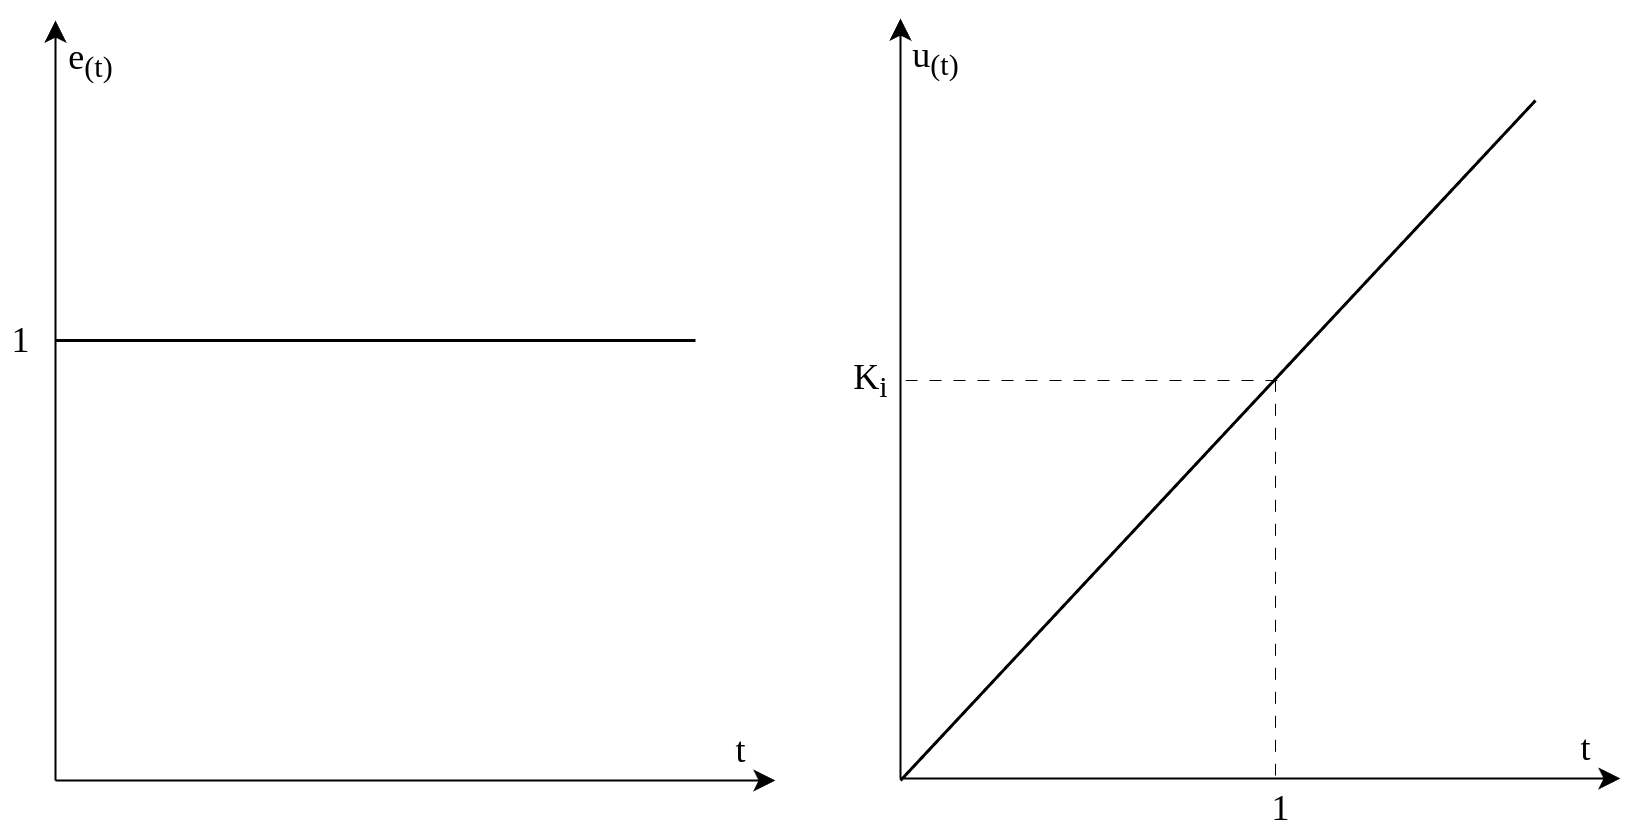
\includegraphics[width=13cm]{figures/i.drawio.png}
    \caption{Одзив I регулатора на одскочни сигнал грешке}
    \label{fig:I_одзив}
\end{figure}

\subsubsection{Диференцијално дејство}
Регулација на основу диференцијалног дејства, односно D регулатори, су настали како би отклонили мане I регулатора, односно, како би убрзали одзив у прелазном режиму и смањили осцилације у устаљеном стању. Управљачки сигнал D регулатора представља извод сигнала грешке по времену, помножен фактором појачања диференцијалног дејства $K_d$[8]:
\begin{equation}
    u_{(t)} = K_d\dfrac{de_{(t)}}{dt}
\end{equation}
Функција преноса D регулатора у комплексном домену је:
\begin{equation}
    G_{d(s)} = \dfrac{U_{(s)}}{E_{(s)}} = K_ds
\end{equation}
При сигналу грешке типа рампа, одзив D регулатора изгледа као на слици 2.3.5.
\begin{figure}[H]
    \centering
    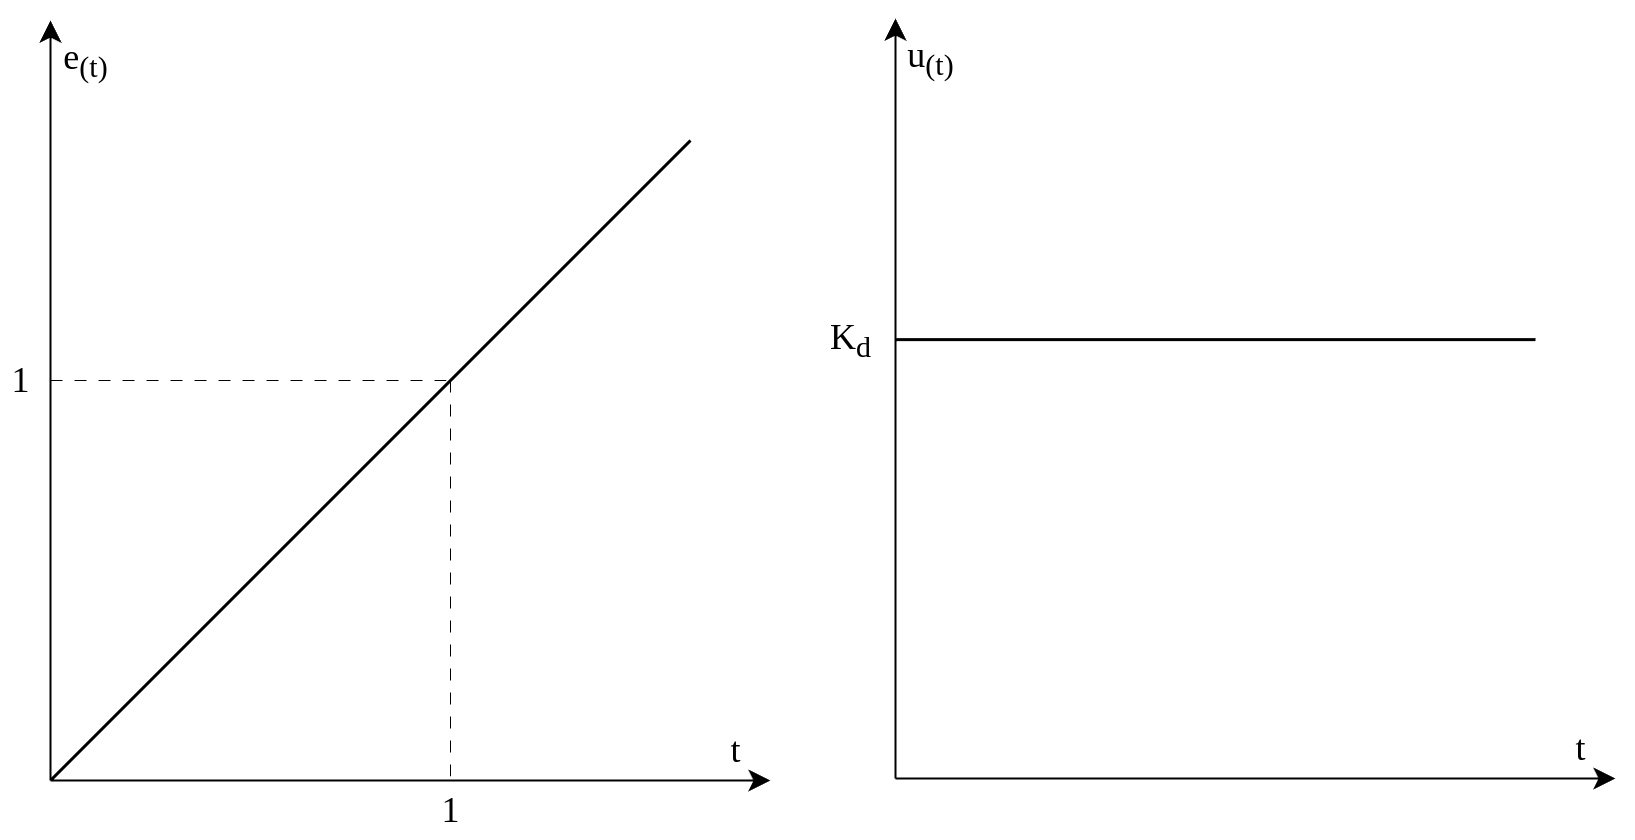
\includegraphics[width=13cm]{figures/d.drawio.png}
    \caption{Одзив D регулатора на сигнал грешке типа рампа}
    \label{fig:D_одзив}
\end{figure}

\subsubsection{PID}
PID регулатор настаје комбиновањем сва три претходно наведена дејства. Подешавањем фактора појачања пропорцијалног, диференцијалног и интегралног дејства могу се обезбедити жељене перформансе система.
Управљачки сигнал PID регулатора је:
\begin{equation}
    u_{(t)} = K_p e_{(t)} + K_i\int_{0}^{t}e_{(t)}dt + K_d\dfrac{de_{(t)}}{dt}
\end{equation}
Функција преноса PID регулатора у комплексном домену је:
\begin{equation}
    G_{pid(s)} = \dfrac{U_{(s)}}{E_{(s)}} = K_p + \dfrac{K_i}{s} + K_ds
\end{equation}
Блок шема која обухвата све 3 дејства PID регулатора је приказана на слици 2.3.6.
\begin{figure}[H]
    \centering
    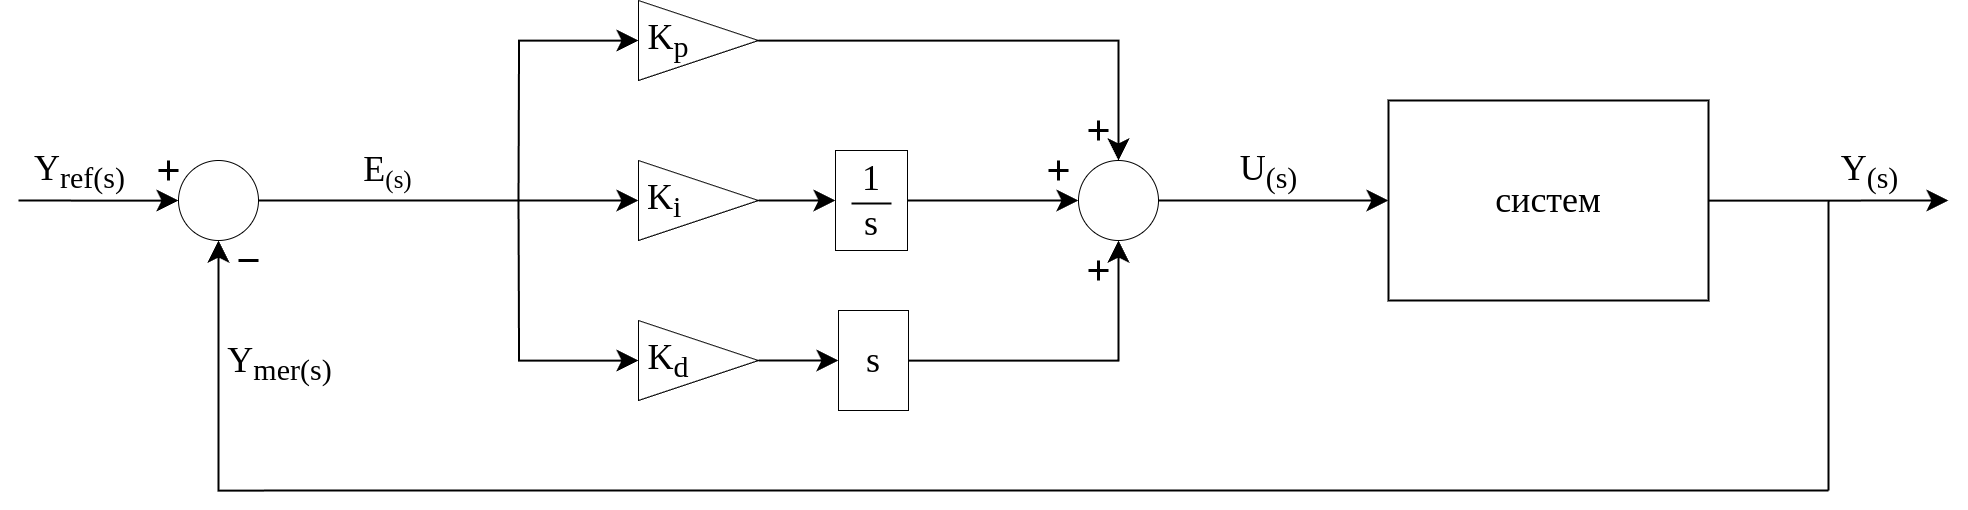
\includegraphics[width=18cm]{figures/pid.drawio.png}
    \caption{Блок шема PID регулатора у затвореној спрези}
    \label{fig:PID_затворена_спрега}
\end{figure}

\subsection{\textit{Particle swarm optimization}}
Оптимизација представља процес одређивања најбољег решења (према једном или више критеријума) у скупу потенцијалних решења. То се постиже дефинисањем циља у облику параметризоване функције $f$, која се назива критеријум оптималности или функција циља, тако да се оптимизација сведе на проналажење вредности параметара који минимизују или максимизују вредност $f$ [9].

PSO (\textit{Particle swarm optimization}), односно оптимизација ројем честица, је метахеуристичка глобална оптимизациона метода, која припада групи алгоритама заснованих на концепту интелигенције ројева [9]. Инспирисана је социјалним понашањем примећеним у јатима риба и птица при потрази за храном. Скуп потенцијалних решења проблема оптимизације је дефинисан као рој честица које могу да се крећу кроз параметарски простор, дефинишући трајекторије које су вођене сопственим и глобалним најбољим учинком.

\subsubsection{Кретање честица}
У PSO алгоритму, свако потенцијално решење се назива честица, и представља тачку у $N$-димензионом простору, где $N$ представља број променљивих у критеријуму оптималности. Позиција $i$-те честице се изражава преко вектора $\vec x_i$:
\begin{equation}
    \vec x_i = [x_{i1} x_{i2} x_{i3}... x_{iN}]^T
\end{equation}
Популација од $M$ честица чини рој:
\begin{equation}
    \textbf{X} = [\vec x_1 \vec x_2 ... \vec x_M]
\end{equation}
При потрази за оптималним решењем, свака честица итеративно дефинише своју трајекторију на основу једначинe кретања:
\begin{equation}
    \vec x_i(t+1) = \vec x_i(t) +\vec v_i(t+1),
\end{equation}
где $t$ и $t+1$ представљају тренутну и наредну итерацију извршавања алгоритма, а $\vec v_i$ представља вектор брзине $i$-те честице. Брзина $i$-те честице у наредној итерацији се рачуна преко формуле:
\begin{equation}
    \vec v_i(t+1) = w\vec v_i(t) + c_p(\vec p_i- \vec x_i(t))R_1(t) + c_g(\vec g- \vec x_i(t))R_2(t),
\end{equation}
где $w$ представља коефицијент инерције, $c_p$ и $c_g$ су когнитивни и социјални коефицијенти, који се заједно називају коефицијенти убрзања, $\vec p_i$ је вектор најбољег решења које је $i$-та честица до сад пронашла, $\vec{g}$ је вектор најбољег решења које је рој до сад пронашао,  $R_1$ и $R_2$ су насумични фактори вредности [0,1].

Из једначине (22) се може уочити да се вектор брзине састоји из 3 компоненте:
\begin{itemize}
    \item инерцијалне,
    \item когнитивне и
    \item социјалне
\end{itemize}
Инерцијална компонента спречава драстичне промене брзине честице. Коефицијент инерције је фактор који контролише инерцију честице регулишући допринос брзине из претходне итерације. Овај фактор утиче на однос експлорације и експлоатације. Веће вредности коефицијента инерције фаворизују глобалну експлорацију, док мање вредности фаворизују локалну експлоатацију. У основној варијанти PSO алгоритма, која је дефинисана изразима (21) и (22), коефицијент инерције је био константан и јединичне вредности, због чега није истицан као посебан параметар [10].

Когнитивна компонента представља тенденцију честица да се врате на своју претходно пронађену најбољу позицију. Социјална компонента представља склоност честица да се крећу ка најбољој позицији целог роја. 
Потребна је одговарајућа равнотежа између вредности ових коефицијената, јер неприкладне вредности могу да резултују дивергентним или цикличним понашањем роја [11]. Како се коефицијенти повећавају, фреквенција осцилација честица око оптимума се повећава, док мање вредности доводе до синусоидалних путања [9][12]. Уколико су коефицијенти једнаки, честице се крећу ка тачки на средини између личног и глобалног најбољег решења [13]. При вредностима $c_p\;>>\;c_g$, лична најбоља позиција има више утицаја на кретање честица, што може довести до претеране експлорације у простору претраге [11]. При вредностима $c_p\;<<\;c_g$, глобална најбоља позиција има више утицаја на кретање честица, што може довести до превремене конвергенције (локалног оптимума) [11]. Коефицијенти убрзања су усвајани по различитим препорукама. Неке од препорука за усвајање вредности су [10]: 
\begin{itemize}
    \item $c_p\;=\;c_g\;=\;2$
    \item $c_p\;=\;c_g\;=\;0.5$
    \item $c_p\;=\;2.8,\;c_g\;=\;1.3$
\end{itemize}
\subsubsection{Модификације PSO алгоритма}
Основна варијанта PSO алгоритма показује задовољавајуће перформансе за једноставније проблеме. Код сложенијих проблема, који обухватају присуство великог броја локалних оптимума и вишедимензионе просторе претраге, основна варијанта није довољно ефикасна [10]. Због тога су уведене бројне модификације.

Често коришћена модификација PSO алгоритма уводи концепт променљиве инерције. Уколико се у почетним итерацијама усвоји висока вредност коефицијента инерције, способност роја да претражи целокупан простор претраге је велика. Како претрага одмиче, вредност инерције се смањује како би се смањивао утицај експлорације, а повећавао утицај експлоатације. То дозвољава честицама да се више крећу на основу сопственог искуства и искуства целог роја, а мање услед сопствене инерције [10]. Најједноставнија имплементација овакве модификације линеарно смањује вредности коефицијента инерције, од почетне вредности $w_{max}=0.9$ до крајње вредности $w_{min}=0.4$. Друге стратегије промељиве инерције обухватају [9]:
\begin{itemize}
    \item насумично мењање коефицијента, коришћењем насумичног параметра $r\in(0,1)$: $w(t)\;=\;0.5\;+\;\dfrac{r}{2}$,
    \item смањивање инерције на основу односа глобалног и локалног оптимума: $w_i(t)\;=\;1.1\;-\;\dfrac{p_i}{g}$,
    \item хаотично смањивање инерције, комбиновањем линеарног смањивања и параметра $z\;=\;4r(1-r)$, где је $r\in(0,1)$ насумичан параметар.
\end{itemize}

Друга модификација уводи концепт ограничавања максималне дозвољене вредности брзине честица. Ова модификација је уведена због дивергенције роја услед неконтролисаног повећања интензитета брзина. Та дивергенција се назива експлозија роја. Вредност максималне брзине, по координатном правцу $i$, се израчунава на основу следећег израза [10]:
\begin{equation}
    v_{max(i)}\;=\;k\cdot min(b_i - a_i),
\end{equation}
где $k$ представља одговарајући коефицијент, а $a_i$ и $b_i$ представљају горњу и доњу границу вредности координата по том правцу. За параметар $k$ се препоручују вредности у опсегу (0.1, 1) [10].

Још једна модификација PSO алгоритма уводи концепт околине. Код неких сложенијих проблема, PSO алгоритам има проблем западања честица у локалне оптимуме. Овај проблем настаје због формирања униформног роја у крајњим фазама алгоритма, што је резултат усмеравања свих честица ка једној глобално откривеној најбољој позицији. Појам околине смањује утицај глобалног сазнања о најбољем решењу, тако што свака честица дели своја сазнања само са честицама у својој околини, уместо са целим ројем. Једина разлика у једначини кретања честица из основног PSO алгоритма и ове модификације се огледа у томе што се глобална најбоља позиција усваја у околини [10]. Околина честица може да се одређује на основу различитих шема, које се називају топологије. Две основне топологије су:
\begin{itemize}
    \item на основу удаљености и
    \item на основу индекса (прстенаста топологија).
\end{itemize}
Основна варијанта PSO алгоритма је глобална и има звездасту топологију.


Блок шема PSO алгоритма која је представљена на слици 2.4.1 приказује целокупан принцип рада алгоритма.

\begin{figure}[H]
    \centering
    \includegraphics[width=14cm]{figures/pso.drawio.png}
    \caption{Блок шема PSO алгоритма}
    \label{fig:PSO_алгоритам}
\end{figure}
\newpage

\section{Имплементација}

\subsection{Петочлани паралелни манипулатор}
Петочлани паралелни манипулатор је равански механизам, који се састоји из 5 сегмената и 5 ротационих зглобова, односно, то је механизам типа 5R. Оса ротације сваког зглоба је нормална на раван у којој се механизам креће. Сегмент 1 је непокретан, односно база. Сегменти 2 и 5 су актуирани помоћу ротационог актуатора и називају се \textit{proximal}. Сегменти 3 и 4 су пасивни и називају се \textit{distal}. Зглоб између пасивних сегмената посматрамо као крајњи ефектор, у наставку TCP (\textit{tool center point}).

 Поседује 2 степена слободе (DOF, \textit{degrees of freedom}), који одговарају положају TCP у равни. Ово значи да врх крајњег ефектора може да се креће дуж \textit{x} и \textit{y} оса координатног система, и да зависи искључиво од положаја актуираних чланова и конфигурације манипулатора.

\subsubsection{Означавање и параметри}
Петочлани паралелни манипулатор, са карактеристичним векторима, је приказан на слици 3.1.1.
\begin{figure}[H]
    \centering
    \includegraphics[width=12cm]{figures/5bar.jpg}
    \caption{Петочлани паралелни манипулатор}
    \label{fig:5bar_manipulator}
\end{figure}

Све ознаке и вредности константних параметара које се користе при моделовању манипулатора су:
\begin{itemize}
    \item $L,\; R,\; A,\; B,\; TCP$ - положаји зглобова
    \item $x_{TCP},\;y_{TCP}$ - координате TCP
    \item $\vec{r_{1L}},\; \vec{r_{1R}},\; \vec{r_{2}},\; \vec{r_{3}},\; \vec{r_{4}}, \;\vec{r_{5}}\;$ - карактеристични вектори
    \item $S_2,\; S_3,\; S_4,\; S_5\;$ - положаји центра маса сегмената
    \item $\theta_2,\; \theta_3,\; \theta_4,\; \theta_5\;$ - оријентација карактеристичних вектора
    \item $\theta_L = \theta_2, \quad \theta_R = \theta_5-\pi\;$ - углови \textit{proximal} сегмената
    \item $\theta_{4R} = \theta_4-\pi\;$ - оријентација сегмента 4 уведена ради лакше кинематичке анализе
    \item $L = 40mm\;$ - дужина базе
    \item $P = 60mm\;$ - дужина \textit{proximal} сегменaта
    \item $D = 90mm\;$ - дужина \textit{distal} сегменaта
    \item $m_P = 100g\;$ - маса \textit{proximal} сегменaта
    \item $m_D = 120g\;$ - маса \textit{distal} сегменaта
    \item $J_{SP} = \dfrac{1}{12} m_P P ^ 2,\quad J_{SD} = \dfrac{1}{12} m_D D ^ 2\;$ - моменти инерција \textit{proximal} и \textit{distal} сегмената за центре маса
    \item $\vec{v}_{TCP},\; \vec{a}_{TCP}\;$ - брзина и убрзање TCP
    \item $v_{xTCP},\;v_{yTCP}$ - $x$ и $y$ компоненте брзине  TCP
    \item $a_{xTCP},\;a_{yTCP}$ - $x$ и $y$ компоненте убрзања TCP
    \item $\omega_L,\; \omega_R,\; \omega_3,\; \omega_4\;$ - интензитети угаоних брзина сегмената
    \item $\alpha_L,\; \alpha_R,\; \alpha_3,\; \alpha_4\;$ - интензитети угаоних убрзања сегмената
    \item $\vec{a}_{S2},\; \vec{a}_{S3},\; \vec{a}_{S4},\; \vec{a}_{S5}\;$ - убрзања центра маса сегмената
    \item $a_{Sx},\; a_{Sy}\;$ - $x$ и $y$ компоненте убрзања центра маса сегмената
    \item $M_L,\;M_R\;$ - улазни обртни моменти
    \item $F_{12x},\; F_{12y}\;$ - $x$ и $y$ компоненте реакције везе којом сегмент 1 делује на сегмент 2
\end{itemize}

\subsubsection{Кинематика}
Директан кинематски модел манипулатора описује како се сви сегменти и TCP крећу у зависности од вредности угла, угаоне брзине и угаоног убрзања улазних сегмената.

Улази у директан кинематски модел су:
\begin{itemize}
    \item $\theta_L, \; \theta_R\;$ - углови,
    \item $\omega_L, \; \omega_R\;$ - угаоне брзине и
    \item $\alpha_L, \; \alpha_R\;$ - угаона убрзања \textit{proximal} сегмената
\end{itemize}
Излази из директног кинематског модела су:
\begin{itemize}
    \item $\theta_3, \; \theta_{4R}\;$ - углови,
    \item $\omega_3, \; \omega_4\;$ - угаоне брзине,
    \item $\alpha_3, \; \alpha_4\;$ - угаона убрзања \textit{distal} сегмената и
    \item $x_{TCP},\;y_{TCP},\; \vec{v}_{TCP},\; \vec{a}_{TCP}\;$ - координате, брзина и убрзање TCP
\end{itemize}

Једначине положаја TCP су:
\begin{equation}
    \vec{r}_{TCP} = \vec{r}_{1L} + \vec{r}_2 + \vec{r}_3
\end{equation}
\begin{equation}
    \vec{r}_{TCP} = \vec{r}_{1R} - \vec{r}_5 - \vec{r}_4
\end{equation}
Пребацивањем у Ојлеров облик и убацивањем параметара постају:
\begin{equation}
    \vec{r}_{TCP} = \dfrac{L}{2}e^{i\pi} + Pe^{i\theta_L} + De^{i\theta_3}
\end{equation}
\begin{equation}
    \vec{r}_{TCP} = \dfrac{L}{2}e^{i0} + Pe^{i\theta_R} + De^{i\theta_{4R}}
\end{equation}
Разлагањем на \textit{x} и \textit{y} компоненте, једначине (26) и (27) постају:
\begin{equation}
    x_{TCP} = -\dfrac{L}{2} + Pcos\theta_L + Dcos\theta_3
\end{equation}
\begin{equation}
    x_{TCP} = \dfrac{L}{2} + Pcos\theta_R + Dcos\theta_{4R}
\end{equation}
\begin{equation}
    y_{TCP} = Psin\theta_L + Dsin\theta_3
\end{equation}
\begin{equation}
    y_{TCP} = Psin\theta_R + Dsin\theta_{4R}
\end{equation}

Једначине (28)-(31) чине систем са 4 непознате: $\theta_3,\;\theta_{4R},\;x_{TCP},\;y_{TCP}$. Решења за $\theta_3,\;\theta_{4R}$ су:
\begin{equation}
    \theta_3 = 2arctg\left(\dfrac{-\dfrac{y_A - y_B}{D} + \sigma_1\sqrt{\left(\dfrac{x_A-x_B}{D}\right)^2+\left(\dfrac{y_A-y_B}{D}\right)^2-\left(\left(\dfrac{x_A-x_B}{D}\right)^2+\left(\dfrac{y_A-y_B}{D}\right)^2\right)^2\dfrac{1}{4}}}{\dfrac{1}{2}\left(\left(\dfrac{x_A-x_B}{D}\right)^2+\left(\dfrac{y_A-y_B}{D}\right)^2\right)-\dfrac{x_A-x_B}{D}}\right)
\end{equation}
\begin{equation}
    \theta_{4R} = 2arctg\left(\dfrac{-\dfrac{y_B - y_A}{D} + \sigma_2\sqrt{\left(\dfrac{x_B-x_A}{D}\right)^2+\left(\dfrac{y_B-y_A}{D}\right)^2-\left(\left(\dfrac{x_B-x_A}{D}\right)^2+\left(\dfrac{y_B-y_A}{D}\right)^2\right)^2\dfrac{1}{4}}}{\dfrac{1}{2}\left(\left(\dfrac{x_B-x_A}{D}\right)^2+\left(\dfrac{y_B-y_A}{D}\right)^2\right)-\dfrac{x_B-x_A}{D}}\right),
\end{equation}
где $\sigma_1=+1$ и $\sigma_2=-1$, представљају избор конфигурације манипулатора. Вредности за $x_{TCP},\;y_{TCP}$ се добијају враћањем (9) и (10) у првобитан систем једначина.

Диференцирањем (28)-(31) добијају се једначине брзине TCP-а:
\begin{equation}
    v_{xTCP} = -Psin\theta_L\omega_L - Dsin\theta_3\omega_3
\end{equation}
\begin{equation}
    v_{xTCP} = -Psin\theta_R\omega_R - Dsin\theta_{4R}\omega_4
\end{equation}
\begin{equation}
    v_{yTCP} = Pcos\theta_L\omega_L + Dcos\theta_3\omega_3
\end{equation}
\begin{equation}
    v_{yTCP} = Pcos\theta_R\omega_R + Dcos\theta_{4R}\omega_4
\end{equation}
Записане у матричној форми су:

\begin{equation}
\begin{bmatrix}
-1 & 0 & -Dsin\theta_3 & 0\\
-1 & 0 & 0 & -Dsin\theta_{4R}\\
0 & 1 & -Dcos\theta_3 & 0\\
0 & 1 & 0 & -Dcos\theta_{4R}\\
\end{bmatrix}
\begin{bmatrix}
v_{xTCP}\\
v_{yTCP}\\
\omega_3\\
\omega_4\\
\end{bmatrix}
=
\begin{bmatrix}
Psin\theta_L\omega_L\\
Psin\theta_R\omega_R\\
Pcos\theta_L\omega_L\\
Pcos\theta_R\omega_R\\
\end{bmatrix}
\end{equation}

Диференцирањем (34)-(37) добијају се једначине убрзања TCP-а:
\begin{equation}
    a_{xTCP} = - Psin\theta_L\alpha_L - Pcos\theta_L\omega_L^2 - Dsin\theta_3\alpha_3 - Dcos\theta_3\omega_3^2
\end{equation}
\begin{equation}
    a_{xTCP} =  - Psin\theta_R\alpha_R - Pcos\theta_R\omega_R^2 - Dsin\theta_{4R}\alpha_4 - Dcos\theta_{4R}\omega_4^2
\end{equation}
\begin{equation}
    a_{yTCP} = Pcos\theta_L\alpha_L - Psin\theta_L\omega_L^2 + Dcos\theta_3\alpha_3 - Dsin\theta_3\omega_3^2 
\end{equation}
\begin{equation}
    a_{yTCP} = Pcos\theta_R\alpha_R - Psin\theta_R\omega_R^2 + Dcos\theta_{4R}\alpha_4 - Dsin\theta_{4R}\omega_4^2
\end{equation}
Записане у матричној форми су:
\begin{equation}
\begin{bmatrix}
1 & 0 & Dsin\theta_3 & 0\\
1 & 0 & 0 & Dsin\theta_{4R}\\
0 & 1 & -Dcos\theta_3 & 0\\
0 & 1 & 0 & -Dcos\theta_{4R}\\
\end{bmatrix}
\begin{bmatrix}
a_{xTCP}\\
a_{yTCP}\\
\alpha_3\\
\alpha_4\\
\end{bmatrix}
=
\begin{bmatrix}
- Psin\theta_L\alpha_L - Pcos\theta_L\omega_L^2 - Dcos\theta_3\omega_3^2\\
- Psin\theta_R\alpha_R - Pcos\theta_R\omega_R^2 - Dcos\theta_{4R}\omega_4^2\\
Pcos\theta_L\alpha_L - Psin\theta_L\omega_L^2 - Dsin\theta_3\omega_3^2\\
Pcos\theta_R\alpha_R - Psin\theta_R\omega_R^2 - Dsin\theta_{4R}\omega_4^2\\
\end{bmatrix}
\end{equation}
У прилогу А је MATLAB функција која служи за израчунавање директне кинематике.

Убрзања центра маса свих сегмената се добијају из векторских једначина које изражавају њихов положај преко карактеристичних вектора:
\begin{equation}
    \vec{r}_{S2} = \vec{r}_{1L} + \dfrac{1}{2}\vec{r}_2
\end{equation}
\begin{equation}
    \vec{r}_{S3} = \vec{r}_{1L} + \vec{r}_2 + \dfrac{1}{2}\vec{r}_3
\end{equation}
\begin{equation}
    \vec{r}_{S4} = \vec{r}_{1R} - \vec{r}_5 - \dfrac{1}{2}\vec{r}_4
\end{equation}
\begin{equation}
    \vec{r}_{S5} = \vec{r}_{1R} - \dfrac{1}{2}\vec{r}_5
\end{equation}
Два пута диференцирамо ове једначине, и затим их разлажемо на  $x$ и $y$ компоненте како би добили изразе за убрзања центра маса:
\begin{equation}
    a_{S2x} = -\dfrac{P}{2}\omega_L^2cos\theta_L - \dfrac{P}{2}\alpha_Lsin\theta_L
\end{equation}
\begin{equation}
    a_{S2y} = -\dfrac{P}{2}\omega_L^2sin\theta_L + \dfrac{P}{2}\alpha_Lcos\theta_L
\end{equation}
\begin{equation}
    a_{S3x} = -P\omega_L^2cos\theta_L - P\alpha_L sin\theta_L - \dfrac{D}{2}\omega_3^2cos\theta_3 - \dfrac{D}{2}\alpha_3sin\theta_3
\end{equation}
\begin{equation}
    a_{S3y} = -P\omega_L^2sin\theta_L + P\alpha_Lcos\theta_L - \dfrac{D}{2}\omega_3^2sin\theta_3 + \dfrac{D}{2}\alpha_3cos\theta_3
\end{equation}
\begin{equation}
    a_{S4x} = -P\omega_R^2cos\theta_R - P\alpha_R sin\theta_R - \dfrac{D}{2}\omega_4^2cos\theta_{4R} - \dfrac{D}{2}\alpha_4sin\theta_{4R}
\end{equation}
\begin{equation}
    a_{S4y} = -P\omega_R^2sin\theta_R + P\alpha_Rcos\theta_R - \dfrac{D}{2}\omega_4^2sin\theta_{4R} + \dfrac{D}{2}\alpha_4cos\theta_{4R}
\end{equation}
\begin{equation}
    a_{S5x} = -\dfrac{P}{2}\omega_R^2cos\theta_R - \dfrac{P}{2}\alpha_Rsin\theta_R
\end{equation}
\begin{equation}
    a_{S5y} = -\dfrac{P}{2}\omega_R^2sin\theta_R + \dfrac{P}{2}\alpha_Rcos\theta_R
\end{equation}

За инверзан кинематски проблем решићемо само систем за положај, јер нам служи само за одређивање почетних и референтних углова манипулатора. За решавање инверне кинематике такође користимо (28)-(31), само што сматрамо да су нам непознате: $\theta_L,\;\theta_R,\;\theta_3,\;\theta_{4R}$. Решавањем само за $\theta_L$ и $\theta_R$ добијамо:
\begin{equation}
    \theta_L = 2arctg\left(\dfrac{1 + \sigma_1\sqrt{1 - \left(\dfrac{\left(x_{TCP}+\dfrac{L}{2}\right)^2 + y_{TCP}^2 + P^2 - D^2}{2y_{TCP}P}\right)^2+\left(\dfrac{x_{TCP}+\dfrac{L}{2}}
    {y_{TCP}}\right)^2}}
    {\dfrac{\left(x_{TCP}+\dfrac{L}{2}\right)^2 + y_{TCP}^2 + P^2 - D^2}{2y_{TCP}P} + \dfrac{x_{TCP}+\dfrac{L}{2}}
    {y_{TCP}}}\right)
\end{equation}
\begin{equation}
    \theta_R = 2arctg\left(\dfrac{1 + \sigma_2\sqrt{1 - \left(\dfrac{\left(x_{TCP}-\dfrac{L}{2}\right)^2 + y_{TCP}^2 + P^2 - D^2}{2y_{TCP}P}\right)^2+\left(\dfrac{x_{TCP}-\dfrac{L}{2}}
    {y_{TCP}}\right)^2}}
    {\dfrac{\left(x_{TCP}-\dfrac{L}{2}\right)^2 + y_{TCP}^2 + P^2 - D^2}{2y_{TCP}P} + \dfrac{x_{TCP}-\dfrac{L}{2}}
    {y_{TCP}}}\right),
\end{equation}
где $\sigma_1=+1$ и $\sigma_2=-1$, представљају избор конфигурације манипулатора.
У прилогу Б је MATLAB функција која служи за израчунавање инверзне кинематике.

\newpage
\subsubsection{Динамика}
На слици 3.1.2 су приказана сва оптерећења која делују на чланове, у облику \textit{Free-Body Diagram}-а.
\begin{figure}[H]
    \centering
    \includegraphics[width=17.5cm]{figures/5bar_fbd.jpg}
    \caption{\textit{Free-Body Diagram} петочланог паралелног манипулатора}
    \label{fig:5bar_fbd}
\end{figure}

Инверзан динамички модел манипулатора описује потребна улазна оптерећења како би се остварило задато кретање.

Њутн-Ојлерове једначине кретања за сваки члан ћемо раставити на $x$ и $y$ компоненте. За члан 2 једначине су:
\begin{equation}
    m_P a_{s2x} = F_{12x}+F_{32x}
\end{equation}
\begin{equation}
    m_P a_{s2y} = F_{12y}+F_{32y}
\end{equation}
\begin{equation}
    J_{SP} \alpha_L = M_L + \dfrac{P}{2}F_{32y}cos\theta_L - \dfrac{P}{2}F_{32x}sin\theta_L - \dfrac{P}{2}F_{12y}cos\theta_L + \dfrac{P}{2}F_{12x}sin\theta_L
\end{equation}
За члан 3:
\begin{equation}
    m_D a_{s3x} = -F_{32x}+F_{43x}
\end{equation}
\begin{equation}
    m_D a_{s3y} = -F_{32y}+F_{43y}
\end{equation}
\begin{equation}
    J_{SD} \alpha_3 = \dfrac{D}{2}F_{43y}cos\theta_3 - \dfrac{D}{2}F_{43x}sin\theta_3 + \dfrac{D}{2}F_{32y}cos\theta_3 - \dfrac{D}{2}F_{32x}sin\theta_3
\end{equation}
За члан 4:
\begin{equation}
    m_D a_{s4x} = -F_{43x}+F_{54x}
\end{equation}
\begin{equation}
    m_D a_{s4y} = -F_{43y}+F_{54y}
\end{equation}
\begin{equation}
    J_{SD} \alpha_4 = - \dfrac{D}{2}F_{54y}cos\theta_{4R} + \dfrac{D}{2}F_{54x}sin\theta_{4R} - \dfrac{D}{2}F_{43y}cos\theta_{4R} + \dfrac{D}{2}F_{43x}sin\theta_{4R}
\end{equation}
За члан 5:
\begin{equation}
    m_P a_{s5x} = -F_{43x}+F_{54x}
\end{equation}
\begin{equation}
    m_P a_{s5y} = -F_{43y}+F_{54y}
\end{equation}
\begin{equation}
    J_{SP} \alpha_R = M_R + \dfrac{P}{2}F_{54y}cos\theta_R - \dfrac{P}{2}F_{54x}sin\theta_R + \dfrac{P}{2}F_{15y}cos\theta_R - \dfrac{P}{2}F_{15x}sin\theta_R
\end{equation}

Пребацивање у матричној форми су:

\scriptsize
\begin{equation}
\textbf{A}=
\begingroup % keep the change local
\setlength\arraycolsep{3pt}
\left[
\begin{array}{cccccccccccc}
1 & 0 & 0 & 1 & 0 & 0 & 0 & 0 & 0 & 0 & 0 & 0 \\
0 & 1 & 0 & 0 & 1 & 0 & 0 & 0 & 0 & 0 & 0 & 0 \\
\dfrac{P}{2}sin\theta_L & -\dfrac{P}{2}cos\theta_L & 1 & -\dfrac{P}{2}sin\theta_L & \dfrac{P}{2}cos\theta_L & 0 & 0 & 0 & 0 & 0 & 0 & 0 \\
0 & 0 & 0 & -1 & 0 & 1 & 0 & 0 & 0 & 0 & 0 & 0 \\
0 & 0 & 0 & 0 & -1 & 0 & 1 & 0 & 0 & 0 & 0 & 0 \\
0 & 0 & -\dfrac{D}{2}sin\theta_3 & \dfrac{D}{2}cos\theta_3 & 1 & -\dfrac{D}{2}sin\theta_3 & \dfrac{D}{2}cos\theta_3 & 0 & 0 & 0 & 0 & 0 \\
0 & 0 & 0 & 0 & 0 & -1 & 0 & 1 & 0 & 0 & 0 & 0 \\
0 & 0 & 0 & 0 & 0 & 0 & -1 & 0 & 1 & 0 & 0 & 0 \\
0 & 0 & 0 & 0 & \dfrac{D}{2}sin\theta_{4R} & -\dfrac{D}{2}cos\theta_{4R} & 1 & \dfrac{D}{2}sin\theta_{4R} & -\dfrac{D}{2}cos\theta_{4R} & 0 & 0 & 0 \\
0 & 0 & 0 & 0 & 0 & 0 & 0 & -1 & 0 & 1 & 0 & 0 \\
0 & 0 & 0 & 0 & 0 & 0 & 0 & 0 & -1 & 0 & 1 & 0 \\
0 & 0 & 0 & 0 & 0 & 0 & 0 & -\dfrac{P}{2}sin\theta_R & \dfrac{P}{2}cos\theta_R & 1 & -\dfrac{P}{2}sin\theta_R & \dfrac{P}{2}cos\theta_R
\end{array}
\right]
\endgroup
\end{equation}
\normalsize

\begin{equation}
\textbf{A}
\begin{bmatrix}
F_{12x}\\
F_{12y}\\
M_L\\
F_{32x}\\
F_{32y}\\
F_{43x}\\
F_{43y}\\
F_{54x}\\
F_{54y}\\
F_{15x}\\
F_{15y}\\
M_R
\end{bmatrix}
=
\begin{bmatrix}
m_Pa_{S2x}\\
m_Pa_{S2y}\\
J_{SP}\alpha_L\\
m_Da_{S3x}\\
m_Da_{S3y}\\
J_{SD}\alpha_3\\
m_Da_{S4x}\\
m_Da_{S4y}\\
J_{SD}\alpha_4\\
m_Pa_{S5x}\\
m_Pa_{S5y}\\
J_{SD}\alpha_R
\end{bmatrix}
\end{equation}

У прилогу В је MATLAB функција која служи за израчунавање инверзне динамике.
Слика 3.1.3 показује имплементацију целокупног модела петочланог манипулатора. Састоји се из 2 блок функције: директне кинематике и инверзне динамике, и њиховог повезивања.

\begin{figure}[H]
    \centering
    \includegraphics[width=15cm]{figures/simulink_manipulator.jpg}
    \caption{Модел манипулатора у \textit{MATLAB Simulink}-у}
    \label{fig:манипулатор_simulink}
\end{figure}

\subsection{Машина једносмерне струје са константном побудом}
МЈС је моделована у нормализованом домену. Како би могли да користимо нормализован модел, потребно је извршити трансформацију у домен стварних вредности, односно, потребно је излазе помножити коефицијентима како би одговарали некој стварној МЈС.

Улази у МЈС су нормализована вредност арматурног напона [-1,1] и реална вредност момента оптерећења која је помножена са реципрочном вредношћу коефицијента како би се добила одговарајућа нормализована вредност. На слици 3.2.1 је представљена имплементација модела МЈС.

\begin{figure}[H]
    \centering
    \includegraphics[width=17.5cm]{figures/mjs_model.jpg}
    \caption{Модел МЈС у \textit{MATLAB Simulink}-у}
    \label{fig:мјс_simulink}
\end{figure}
Вредности свих параметара модела МЈС су:
\begin{itemize}
    \item $R_a\;=\;0.075\;r.j$
    \item $T_a\;=\;1\;ms$
    \item $psi\_f\;=\;1-R_a\;=\;0.925\;r.j$
    \item $T_m\;=\;0.5\;s$
    \item $B_m\;=\;1\cdot10^{-6}\;r.j$
    \item $Koef\_m\;=\;4.2\;Nm$
    \item $Koef\_w\;=\;12\;\dfrac{rad}{s}$
\end{itemize}
При одскочној вредности арматурног напона у почетном тренутку симулације брзина МЈС има одзив као на слици 3.2.2. У петој секунди симулације, уведен је и поремећај у виду одскочне вредности момента оптерећења.
\begin{figure}[H]
    \centering
    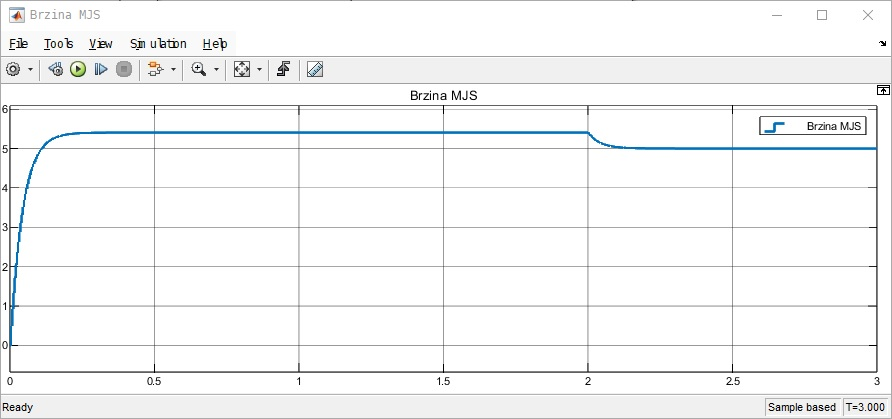
\includegraphics[width=15cm]{figures/brzina_mjs.jpg}
    \caption{Одзив брзине МЈС при одскочној вредности арматурног напона и са одскочним поремећајем момента оптерећења}
    \label{fig:брзина_мјс}
\end{figure}

\subsection{Регулација}
Блок шема принципа регулације манипулатора се састоји из:
\begin{itemize}
    \item Блока за инверзну кинематику који генерише референцу улазних углова,
    \item PID функцијског блока за оба улазна угла који генерише управљачке сигнале,
    \item Леве и десне МЈС, које на основу управљачког сигнала генеришу кретање и
    \item Модела манипулатора.
\end{itemize}
Та блок шема је приказана на слици 3.3.1
\begin{figure}[H]
    \centering
    \includegraphics[width=17.5cm]{figures/regulacija.jpg}
    \caption{Блок шема регулације}
    \label{fig:регулација}
\end{figure}

PID регулатор је имплементиран као \textit{MATLAB Simulink} блок са преносном функцијом: 
\begin{equation}
    G_{PID(s)} \;=\; K_{(1)} \;+\; K_{(2)}\;\dfrac{1}{s} \;+\; K_{(3)}\;\dfrac{N}{1+N\dfrac{1}{s}},
\end{equation}
где $K_{(1)}, \; K_{(2)}$ и $K_{(3)}$ представљају $K_P, \; K_I $ и $ K_D$, а $N$ је коефицијент филтрирања $D$ дејства. На излазу PID блока је прикључен блок сатурације, који ограничава вредност управљачког сигнала на [-1,1].

\subsection{Критеријум оптималности}
Критеријум оптималности је имплементиран као интеграл тежинске суме 2 функције:
\begin{equation}
    f\;=\;\int{w_{(1)}F_{(1)}\;+\;w_{(2)}F_{(2)}},
\end{equation}
где $w_{(i)}$ представља тежински фактор $i$-те подинтегралне функције $F_{(i)}$. Прва подинтегрална функција је:
\begin{equation}
    F_{(1)}\;=\;t(|e_{\theta_L}|\;+\;|e_{\theta_R}|),
\end{equation}
и представља производ збира апсолутних вредности грешака улазних углова и времена. Оптимизовање по овој функцији минимизује укупну грешку улазних углова у стационарном стању.

Друга подинтегрална функција је:
\begin{equation}
    F_{(2)}\;=\;|\Laplace^{-1}\{a_{TCP}\;\dfrac{s}{0.001s+1}\}|,
\end{equation}
и представља апсолутну вредности апроксимације трзаја TCP-а. Оптимизовање по овој функцији минимизује промене убрзања TCP-а, и резултат тога је сигнал без осцилација и прескока [ovde].

Избором вредности тежинских фактора можемо добити задовољавајући резултат оптимизације. Имплементација критеријума оптималности у \textit{MATLAB Simulink}-у је приказана на слици 3.4.1.
\begin{figure}[H]
    \centering
    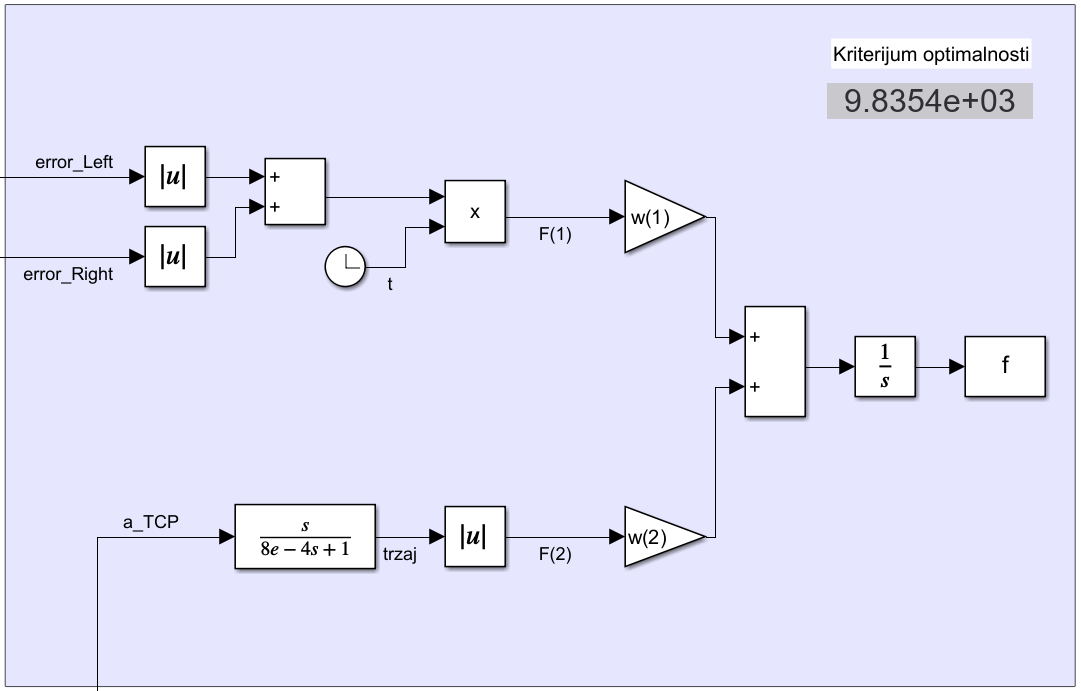
\includegraphics[width=17.5cm]{figures/krit_opti.png}
    \caption{Имплементација критеријума оптималности у \textit{MATLAB Simulink}-у}
    \label{fig:kriterijum_optimalnosti}
\end{figure}
TODO: бољу слику, јер се ова пореметила

\newpage
\section{Резултати и Дискусија}
За оптимизацију је коришћен PSO алгоритам са линеарно смањујућим инерцијалним коефицијентом, са почетном вредношћу $w_{max}=0.9$ и крајњом $w_{min}=0.4$. Коришћена је локална варијанта алгоритма, са околином прстенасте топологије, при чему околину формира $\dfrac{1}{4}$ роја. Усвојене су вредности коефицијената убрзања $c_p\;=\;2.8,\;c_g\;=\;1.3$.

При оптимизацији параметара коришћена је путања средње дужине. Почетна тачка има координате (40mm, 60mm), a крајња (-40mm, 60mm).
Укупно време симулације је $10 s$, а корак симулације је $2 ms$. Такође је уведен и поремећај у виду одскочног спољашњег оптерећења који делује на улазне сегменте, и који започиње у петој секунди симулације.

Извршена је оптимизација са 30 честица и 100 укупних итерација. Такође је тестирано и како мањи број честица и мањи број итерација утиче на резултат оптимизације.
\subsection{Симулација са неоптимизованим параметрима}
При почетним вредностима PID параметара: $K_P=1\;,\;K_I=0\;,\;K_D=0$, одзив левог и десног улазног угла изгледа као на слици 4.1.1. Путања којом се TCP креће је дата на слици 4.1.2.
\begin{figure}[H]
    \centering
    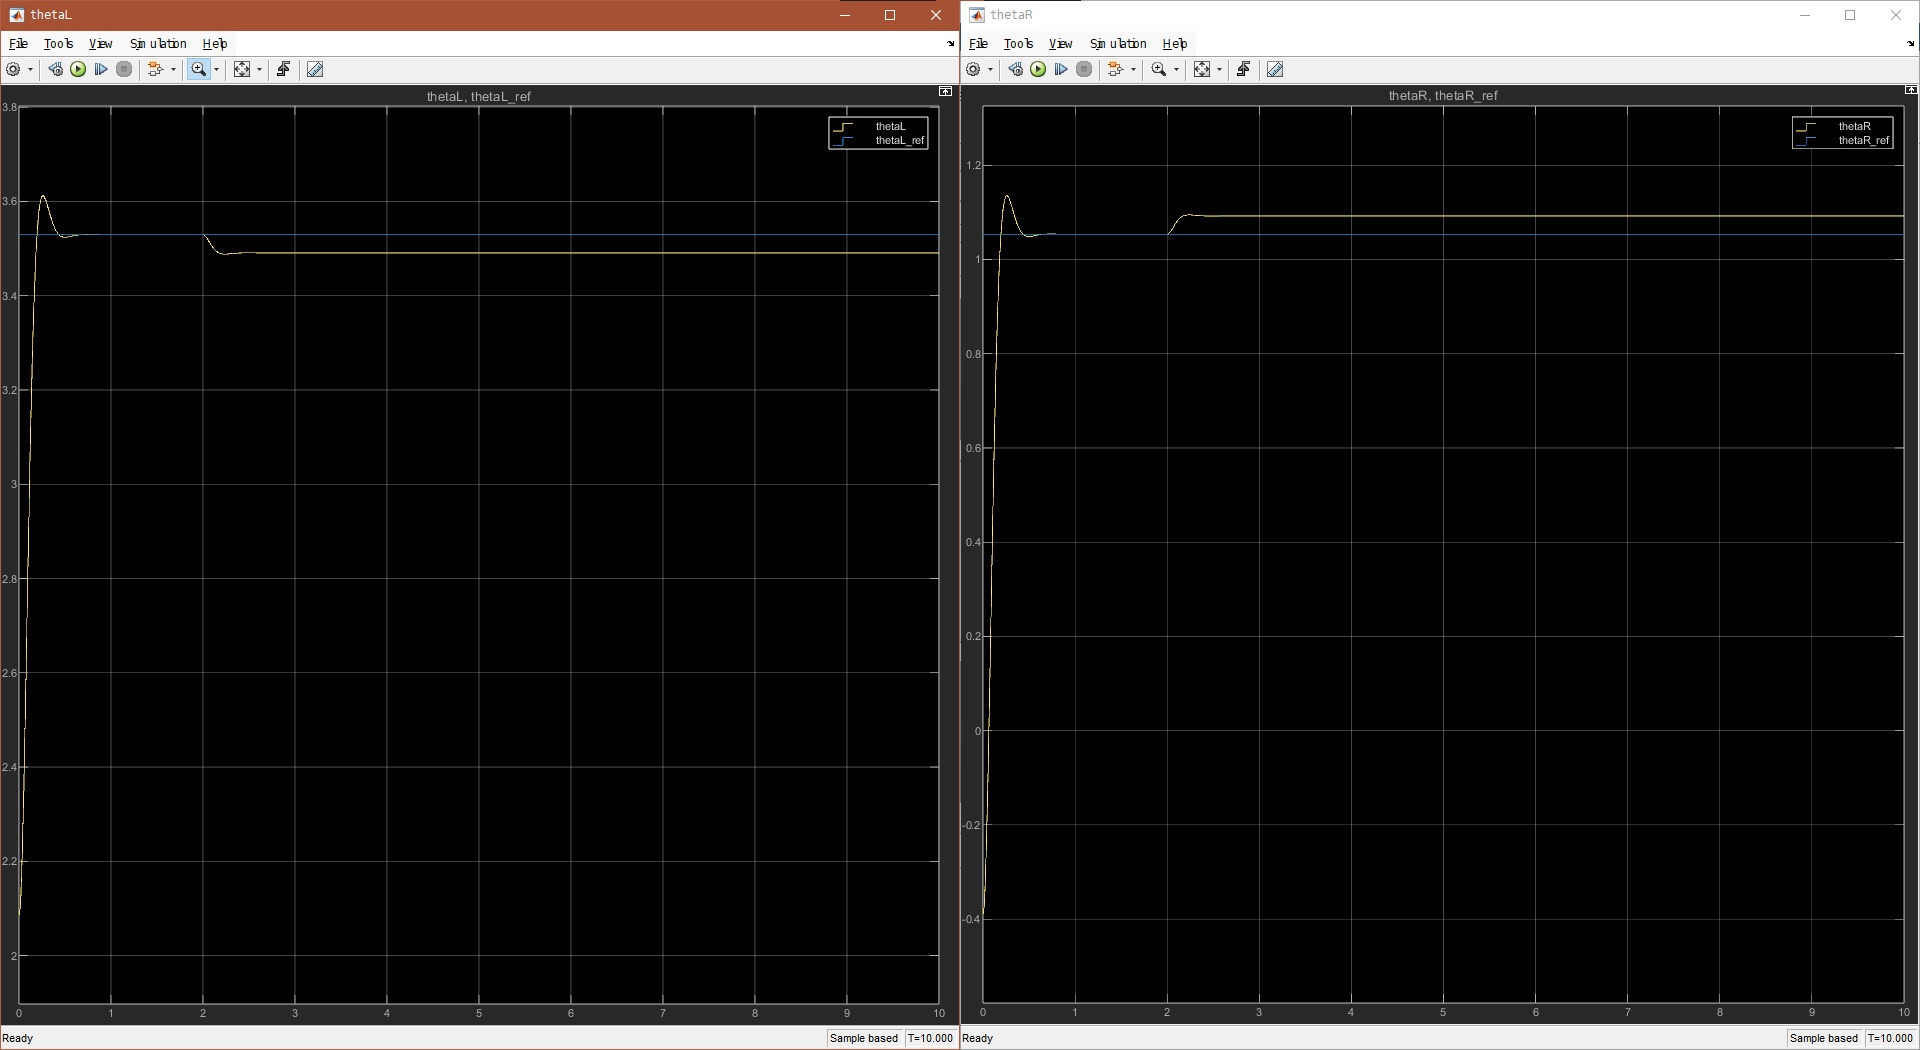
\includegraphics[width=17.5cm]{figures/theta_neopti.jpg}
    \caption{Одзив улазних углова при неоптимизованим параметрима}
    \label{fig:theta_neopti}
\end{figure}
\begin{figure}[H]
    \centering
    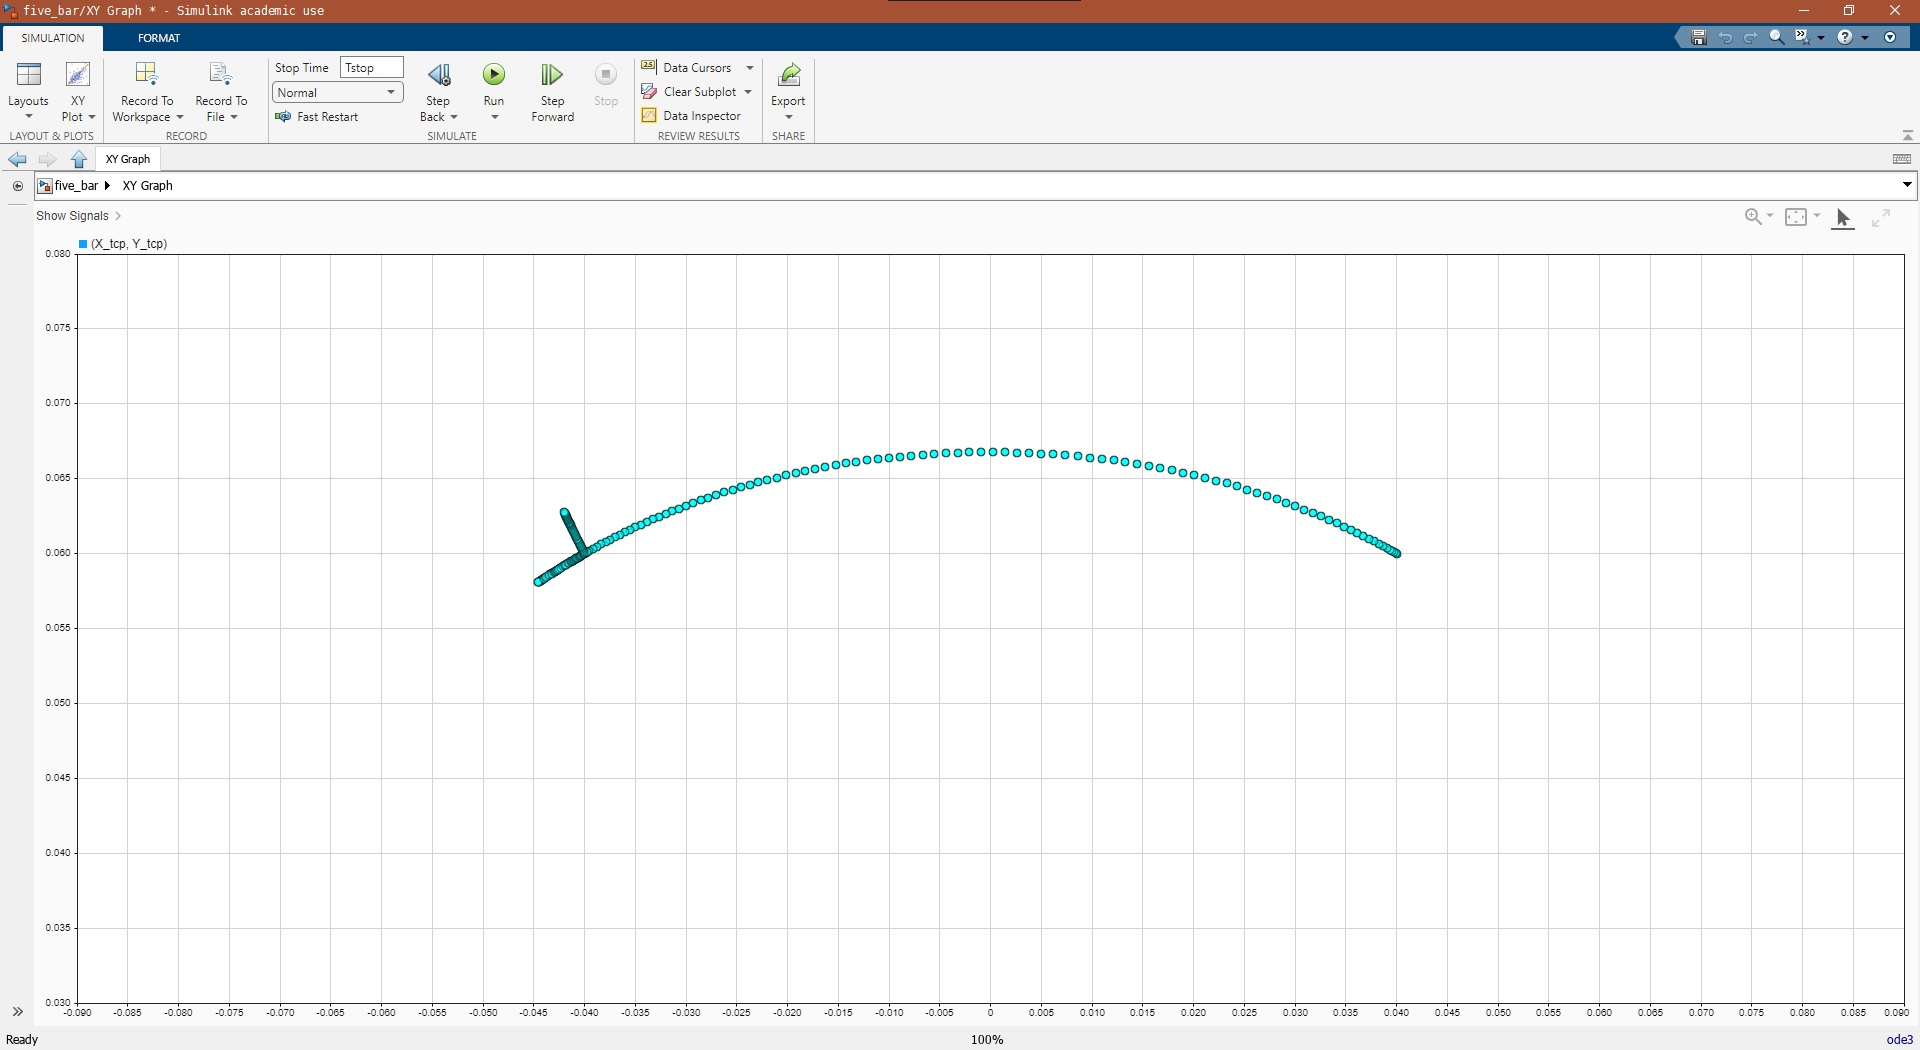
\includegraphics[width=17.5cm]{figures/xy_neopti.jpg}
    \caption{Путања TCP-a при неоптимизованим параметрима}
    \label{fig:xy_neopti}
\end{figure}

Одзив оба улазна угла има прескок и пригушене осцилације. Због тога TCP показује осцилаторно понашање са прескоком пре стабилизације у жељеном положају. Због недостатка I дејства регулатора, овакав систем нема могућност компензовања поремећаја, што је разлог постојања грешке у стационарном стању.

\subsection{Оптимизација параметара са производом апсолутне грешке и времена као јединим критеријумом}
Како би посматрали производ апсолутне грешке и времена као једини критеријум оптималности, потребно је вредност другог тежинског фактора изједначити са нулом. Одзив улазних углова је приказан на слици 4.2.1. TCP описује путању која је дата на слици 4.2.2. На слици 4.2.3 је графички приказ промене најбоље вредности критеријума оптималност по итерацијама алгоритма.

\begin{figure}[H]
    \centering
    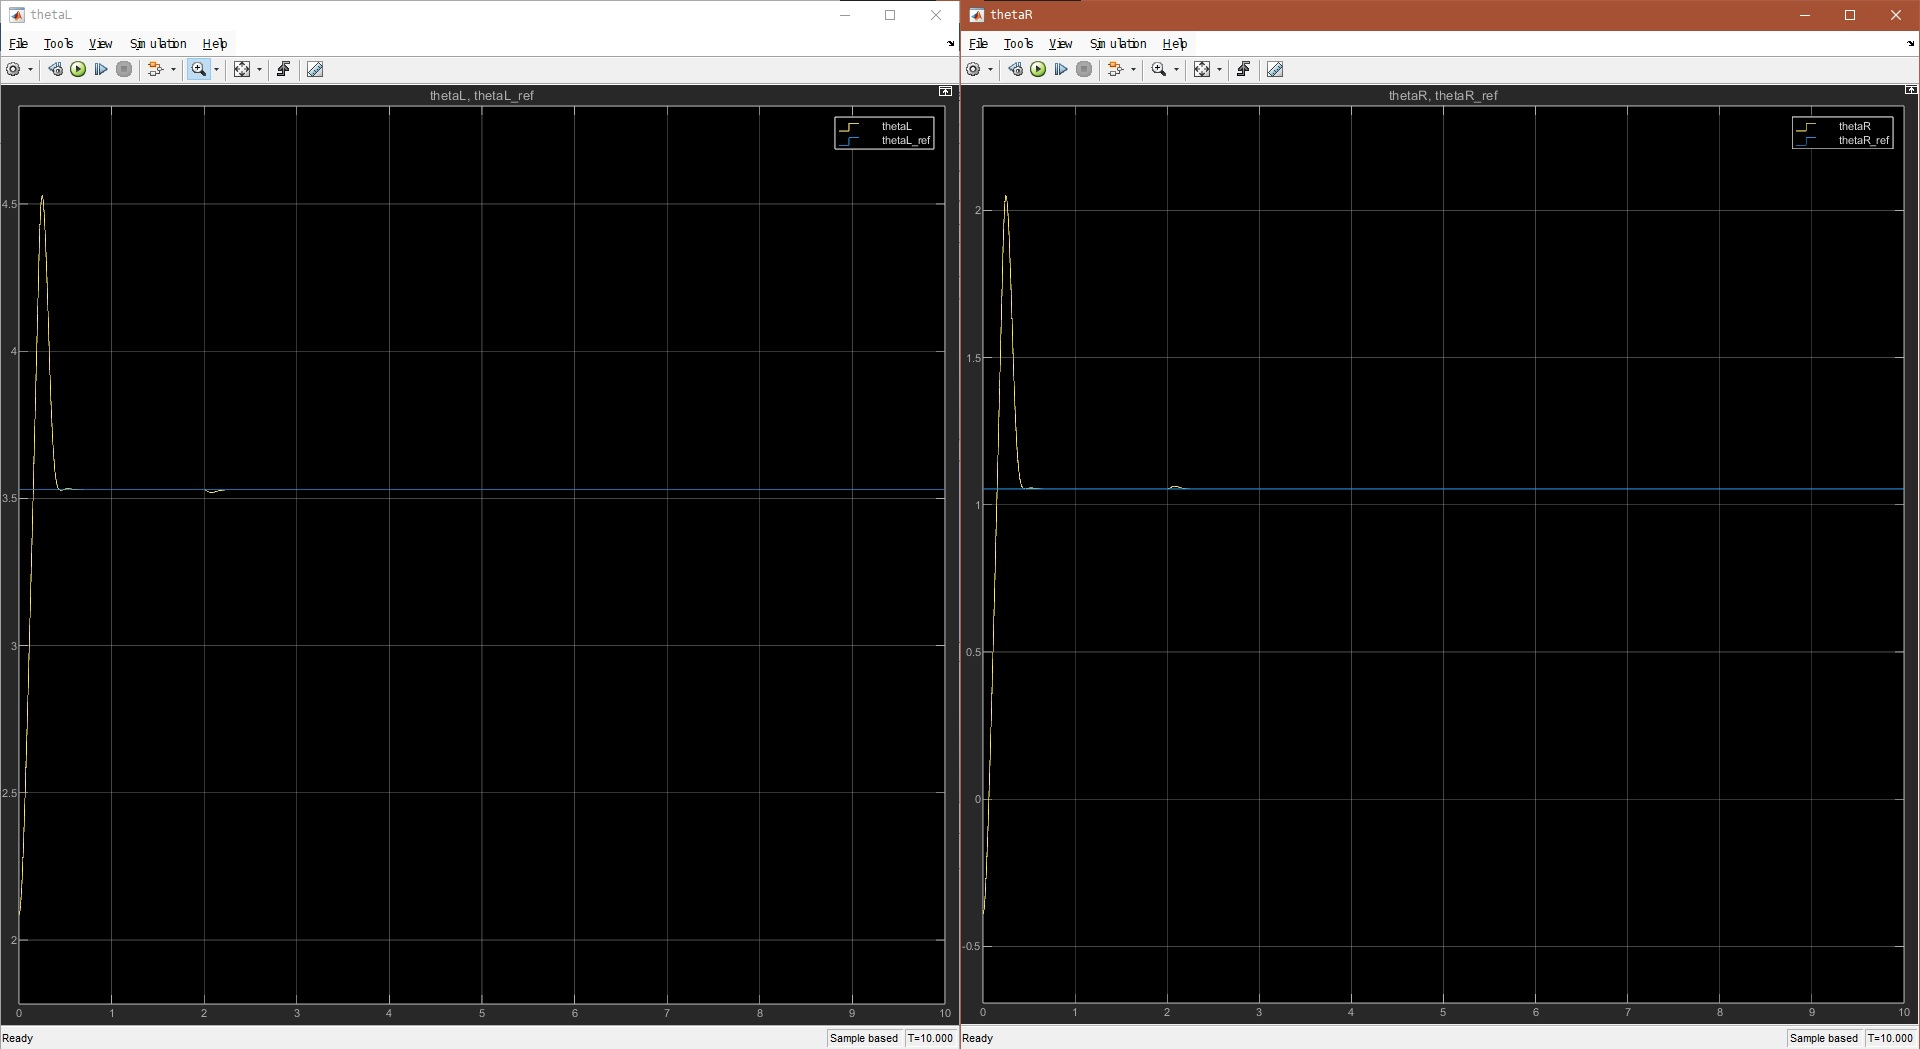
\includegraphics[width=17.5cm]{figures/theta1.jpg}
    \caption{Одзив улазних углова са параметрима оптимизованим по интегралу производа апсолутне грешке и времена као јединим критеријумом}
    \label{fig:w1_0_0_theta}
\end{figure}
\begin{figure}[H]
    \centering
    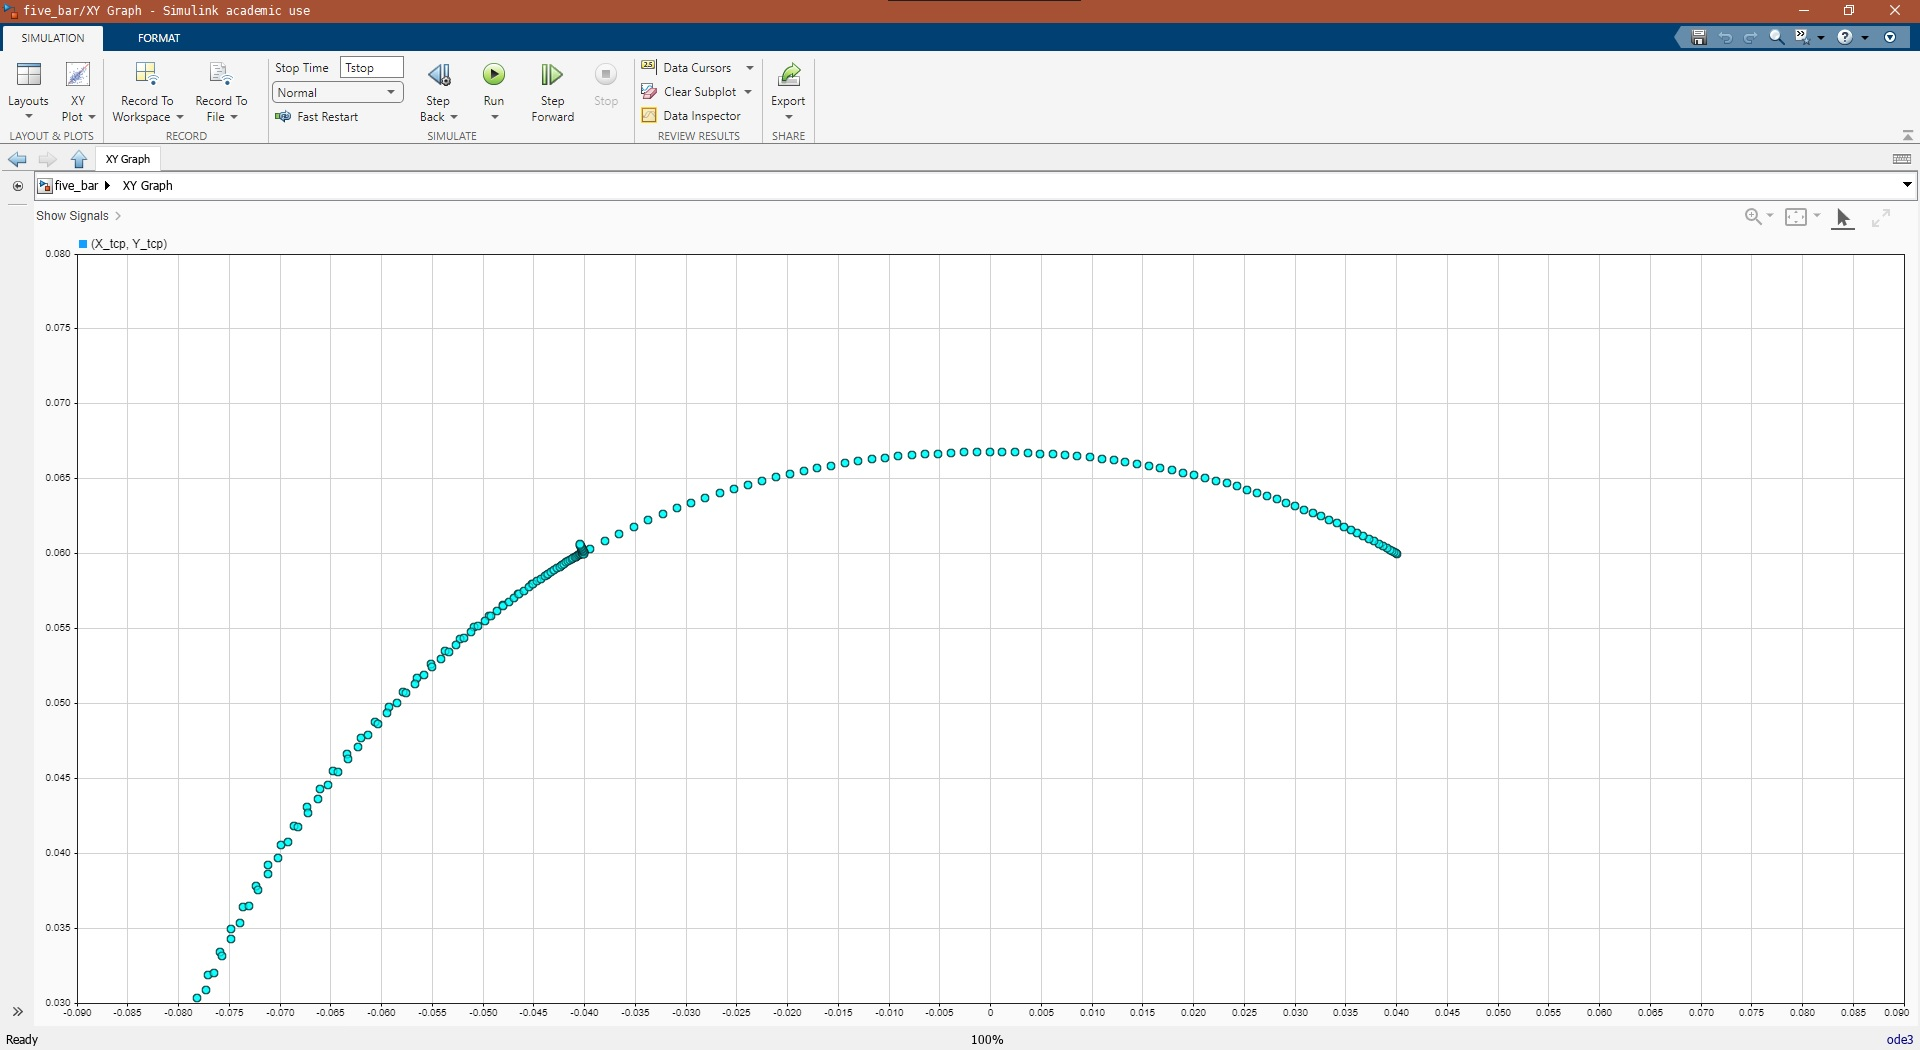
\includegraphics[width=17.5cm]{figures/xy1.jpg}
    \caption{Путања TCP-a са параметрима оптимизованим по интегралу производа апсолутне грешке и времена као јединим критеријумом}
    \label{fig:w1_0_0_xy}
\end{figure}
\begin{figure}[H]
    \centering
    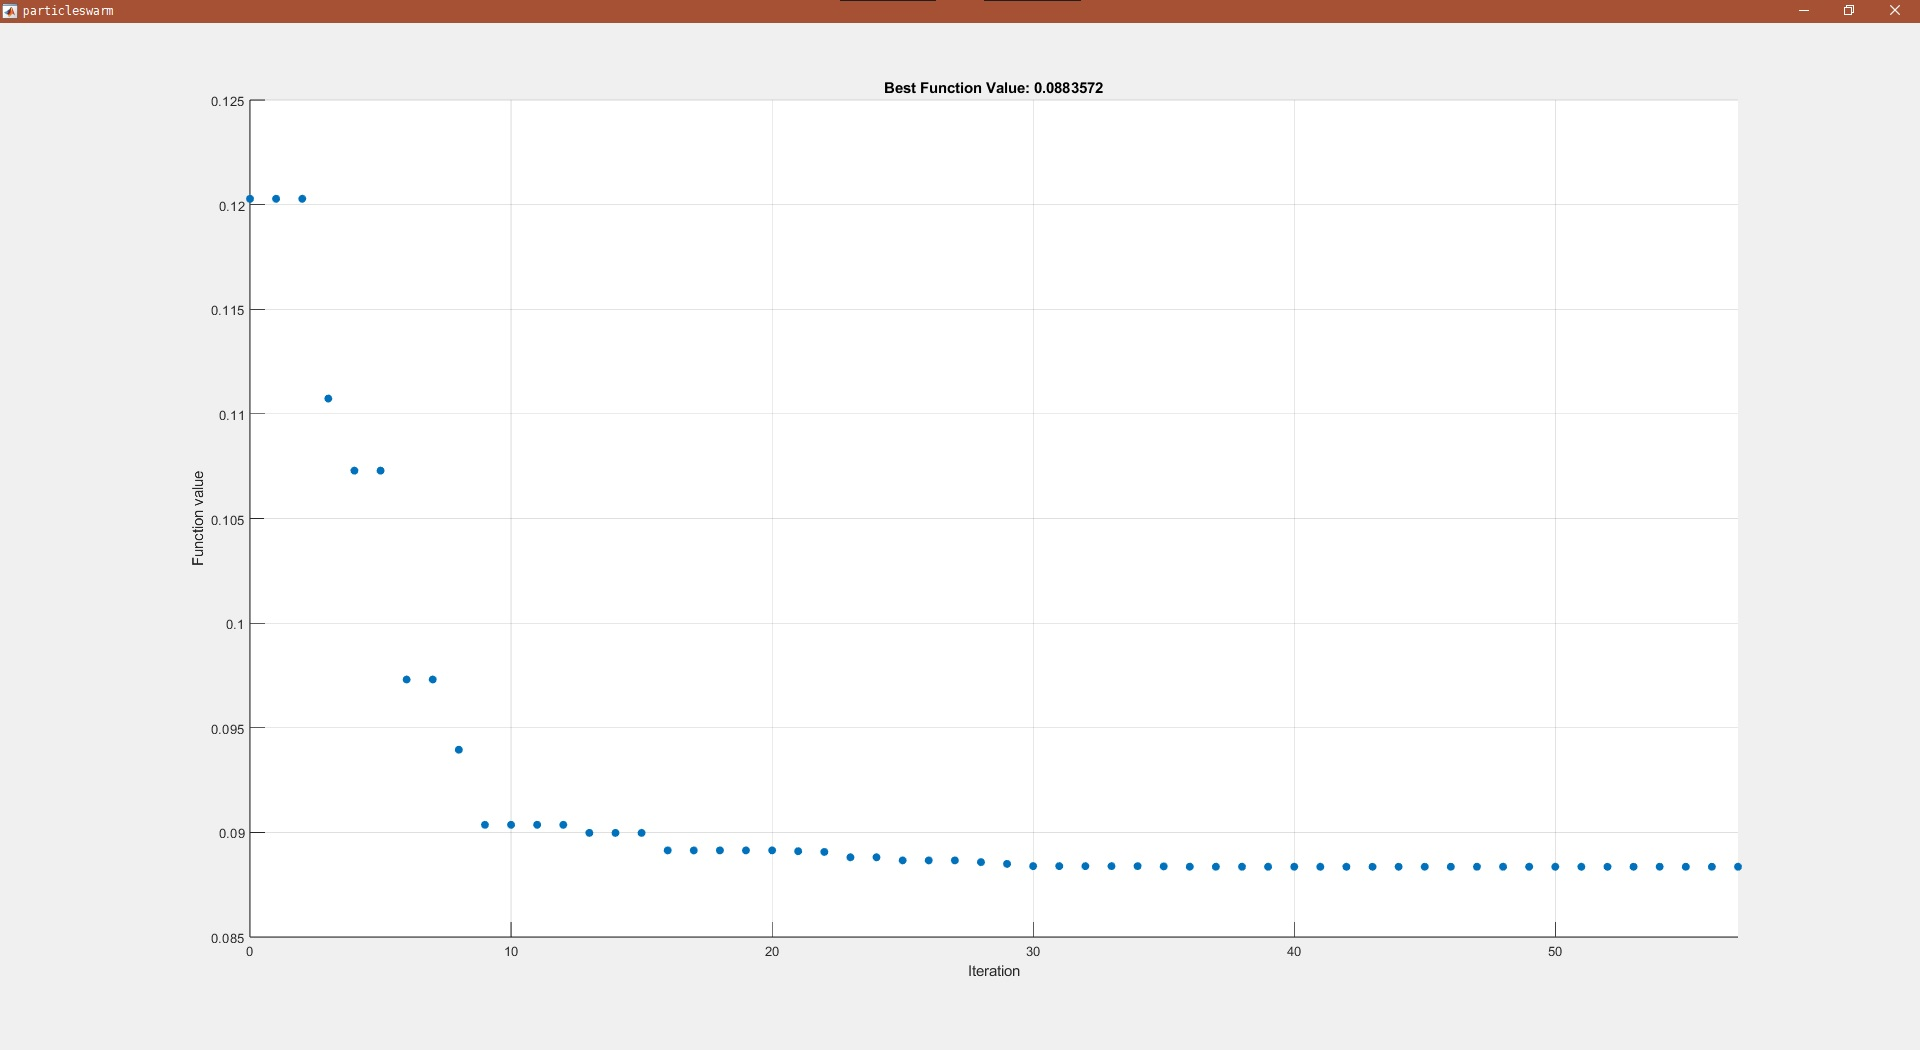
\includegraphics[width=17.5cm]{figures/trend1.jpg}
    \caption{Графички приказ промене најбоље вредности критеријума оптималности}
    \label{fig:trend_1}
\end{figure}
Добијене вредности PID параметара су: $K_P=3.8\;,\;K_I=36\;,\;K_D=0.061$. Одзив улазних углова има велики прескок. Због велике вредности I дејства спољашњи поремећај има само краткотрајан утицај на одзив. Грешка услед њега је брзо отклоњена и TCP се враћа у жељени положај.

\subsection{Оптимизација параметара са становишта трзаја и апсолутне грешке}
Оптимизација по првој подинтегралној функцији не даје задовољавајући одзив. Прескок позиције TCP-а није дозвољен, због чега је потребно променити критеријум оптимизације.
Како би за оптимизацију користили и преосталу подинтегралну функцију, потребно је да се вредности оба тежинска фактора разликује од нуле. Експериментално су одређене њихове вредности како би оптимизацијом добили задовољавајући одзив и износе $w=[50000,\; 1]$. На слици 4.3.1 су приказани одзиви улазних углова. На слици 4.3.2 је дата путања коју TCP описује. На слици 4.3.3 је графички приказ промене најбоље вредности критеријума оптималност по итерацијама алгоритма.

\begin{figure}[H]
    \centering
    \includegraphics[width=17.5cm]{figures/theta2.jpg}
    \caption{Одзив улазних углова са оптимизованим параметрима}
    \label{fig:theta2}
\end{figure}
\begin{figure}[H]
    \centering
    \includegraphics[width=17.5cm]{figures/xy2.jpg}
    \caption{Путања TCP-a са оптимизованим параметрима}
    \label{fig:xy2}
\end{figure}
\begin{figure}[H]
    \centering
    \includegraphics[width=17.5cm]{figures/trend2.png}
    \caption{Графички приказ промене најбоље вредности критеријума оптималности}
    \label{fig:trend_2}
\end{figure}
Добијене вредности PID параметара су: $K_P=28.76\;,\;K_I=0.187\;,\;K_D=0.59$. Оптимизацијом параметара са становишта апсолутне грешке и трзаја даје задовољавајући одзив. Улазни углови немају ни прескок ни осцилације. Спољашњи поремећај не уноси грешку у стационарном стању. 

\subsection{Провера добијених параметара}
Одзив манипулатора са добијеним PID параметрима је оптималан за путању на којој је вршена оптимизација.
Како би проверили да ли добијене вредности параметара задовољавају и при другим путањама, изабране су још 2 путање за тестирање. Прва од тих је значајно дужа, са почетним координатама (80mm, 40mm) и крајњим (-80mm, 40mm). Друга је значајно краћа,  са почетним координатама (10mm, 60mm) и крајњим (-10mm, 60mm).

Одзив улазних углова при дугачкој путањи за тестирање је приказан на слици 4.4.1, док је на слици 4.4.2 приказана путања коју TCP описује.
\begin{figure}[H]
    \centering
    \includegraphics[width=17.5cm]{figures/theta3.jpg}
    \caption{Одзив улазних углова са оптимизованим параметрима при дугачкој путањи}
    \label{fig:theta3}
\end{figure}
\begin{figure}[H]
    \centering
    \includegraphics[width=17.5cm]{figures/xy3.jpg}
    \caption{Путања TCP-a са оптимизованим параметрима}
    \label{fig:xy_3}
\end{figure}
Одзив улазних углова при краткој путањи за тестирање је приказан на слици 4.4.3, док је на слици 4.4.4 приказана путања коју TCP описује.
\begin{figure}[H]
    \centering
    \includegraphics[width=17.5cm]{figures/theta4.jpg}
    \caption{Одзив улазних углова са оптимизованим параметрима при краткој путањи}
    \label{fig:theta_short}
\end{figure}
\begin{figure}[H]
    \centering
    \includegraphics[width=17.5cm]{figures/xy4.png}
    \caption{Путања TCP-a са оптимизованим параметрима}
    \label{fig:xy_short}
\end{figure}

Одзив при обе путање за тестирање је задовољавајући. Грешка у стационарном стању услед поремећаја износи $0.001rad$ за обе путање. При краткој путањи, одзив у прелазном режиму има благе осцилације.


\subsection{Дискусија о утицају броја итерација и броја честица}
При оптимизацији са 30 честица и 10 итерација, фазе експлорације и експлоатације су знатно краће него при оптимизацији са 100 итерација. Последица краће експлорације је већа шанса западања резултата у локални оптимум. Последица краће експлоатације је резултат који се налази близу оптимума али није оптимум, односно превремено прекинута оптимизација.

Тај закључак потврђује резултат оптимизације. Одзив који је добијен приликом оптимизације са 10 итерација изгледа веома слично одзиву са параметрима при оптимизацији са 100 итерација. Вредност критеријума оптималности је мало већа. Вредности добијених PID параметара су: $K_P=6.29\;,\;K_I=0.1\;,\;K_D=1.62$. Због велике разлике PID параметара добијених оптимизацијом са 10 и 100 честица, закључујемо да је добијена вредност локални оптимум. На слици 4.5.1 је дат графички приказ промене најбоље вредности критеријума оптималности, при оптимизацији са 10 итерација.

\begin{figure}[H]
    \centering
    \includegraphics[width=17.5cm]{figures/trend3.jpg}
    \caption{Графички приказ промене најбоље вредности критеријума оптималности, при оптимизацији са 10 итерација}
    \label{fig:trend_3}
\end{figure}

Када смањимо број честица у оптимизацији, смањујемо и могућност алгоритма да претражи цео параметарски простор. Последица тога су смањене шансе алгоритма да пронађе глобални оптимум.

Оптимизацијом са малим бројем честица и 100 итерација су добијене вредности PID параметара: $K_P=30.79\;,\;K_I=0.29\;,\;K_D=0.41$. Слично као и код оптимизације са мањим бројем итерација, резултат представља локални оптимум. Разлика је што оптимизација није превремено прекинута. На слици 4.5.2 је графички приказ промене најбоље вредности критеријума оптималности.

\begin{figure}[H]
    \centering
    \includegraphics[width=17.5cm]{figures/trend4.jpg}
    \caption{Графички приказ промене најбоље вредности критеријума оптималности, при оптимизацији са 5 честица}
    \label{fig:trend_4}
\end{figure}
\newpage

\section{Закључак}
\begin{itemize}
    \item генерално о раду: циљ и шта је урађено
    \item зашто баш тај критеријум оптималности
    \item сумирање резултата
    \item шта може да се унапреди: више путања за оптимизацију због грешака, каскадна регулација електромоторног погона, критеријум оптималности који обухвата и друге функције (нпр. утрошену енергију, глаткост путање), структурна оптимизација, прелазак манипулатора кроз сингуларитете у друге конфигурације, генерисање путање, избегавање препрека
\end{itemize}

Циљ овог рада је да прикаже принцип коришћења PSO алгоритма за пројектовање оптималног управљања паралелним манипулатором. Основни захтеви за оптимално управљање подразумевају:
\begin{itemize}
    \item способност регулатора да што пре доведе манипулатор у жељени положај и
    \item глатку кретњу TCP-а, односно кретњу без прескока и осцилација.
\end{itemize}

Како би оптимизацијом добили одзив система који задовољава захтеве за оптималну кретњу, потребно је захтеве превести у критеријум оптималности. То је урађено интегралом збира две функције. Прва функција обухвата време и грешке улазних углова, чијом минимизацијом задовољавамо први захтев. Друга функција обухвата трзај и њеном минимизацијом добијамо глатку кретњу TCP-а, односно задовољавамо други захтев. Како би могли да добијемо одзив који задовољава оба захтева потребно је подесити тежинске коефицијенте којима се множе вредности функција.

 



\newpage
\section{Прилог}
\subsection{Прилог А}
\begin{figure}[H]
    \centering
    \includegraphics[width=17.5cm]{figures/forward_kinematics.jpg}
    \caption{Функција за директну кинематику у \textit{MATLAB}-у}
    \label{fig:direktna_kinematika_matlab}
\end{figure}
\subsection{Прилог Б}
\begin{figure}[H]
    \raggedright
    \includegraphics[width=8cm]{figures/inverse_kinematics.jpg}
    \caption{Функција за инверзну кинематику у \textit{MATLAB}-у}
    \label{fig:inverzna_kinematika_matlab}
\end{figure}
\subsection{Прилог В}
\begin{figure}[H]
    \raggedright
    \includegraphics[width=16.2cm]{figures/inverse_dynamics.jpg}
    \caption{Функција за инверзну динамику са убрзањима центара маса у \textit{MATLAB}-у}
    \label{fig:inverzna_dinamika_matlab}
\end{figure}

\newpage
\section{Литература}
\begin{enumerate}[start=1,label={[\arabic*]}]
\item J. P. Merlet, Parallel Robots, 2nd ed. Springer 2006
\item \url{https://new.abb.com/en}
\item \url{http://mehanizacija.ftn.uns.ac.rs/wp-content/uploads/2021/02/7.-DINAMICKA-ANALIZA-mehatronika-2019.pdf}, Механика машина, др М. Чавић, редовни професор, МСц Д. Чавић, асистент
\item D. K. Sen, A. Yildiz, O. Kopmaz, "Optimal Design of a Five-Bar Planar Manipulator and Its
Controller by Using Different Algorithms for Minimum
Shaking Forces and Moments for the Largest Trajectory in a
Usable Workspace", MDPI, Machines 2022, 10, 971.
\item \url{https://www.keep.ftn.uns.ac.rs/regulisani-elektromotorni-pogoni/specifikacija/specifikacija-predmeta/}, Регулисани електромоторни погони, др Д. Марчетић, редовни професор, МСц В. Поповић, доцент
\item \url{https://support.maxongroup.com/hc/en-us/articles/360013761160-Motor-data-and-simulation}
\item др Д. Јеркан, Б. Вујков, Збирка задатака из електричних машина за студијски програм мехатроника, Нови Сад, ФТН 2020
\item \url{http://www.automatika.ftn.uns.ac.rs/images/predmeti/Sistemi%20automatskog%20upravljanja%20-%20mehatronika/Predavanja/10_Regulacija.pdf}, Системи аутоматског управљања,
др А. Ристић, редовни професор, др В. Бугарски, доцент
\item F. Marini, B. Walczak, "Particle swarm optimization (PSO). A tutorial", Elsevier 2015
\item Ж. Кановић, З. Јеличић, М. Рапаић, Еволутивни оптимизациони алгоритми у инжењерској пракси, Нови Сад, ФТН 2017
\item M. Jain, V. Saihjpal, N. Singh, S.B. Singh, "An Overview of Variants and Advancements of PSO Algorithm", MDPI, Applied Sciences 2022, 12, 8392.
\item M.R. Bonyadi, Z. Michalewicz, "Impacts of coefficients on movement patterns in the particle swarm optimization algorithm", IEEE Transactions on Evolutionary Computation, 2017, 21, 3
\item S. Rehman, S.A. Khan, L.M. Alhems, "The Effect of Acceleration Coefficients in Particle Swarm Optimization Algorithm with Application to Wind Farm Layout Design", FME Transactions, 2020, 48, 4
\item P. Huang, Y. Xu, B. Liang, "Global minimum-jerk trajectory planning of space manipulator", Int. J. Control. Autom. Syst. 2006, 4, 405–413
\end{enumerate}

\end{document}
